\chapter{La Commune au coeur de l'imaginaire de Masson et Aragon}

\section{Héritage d’André Masson de la Commune de Paris}

\subsection{Article \emph{André Masson et la Commune} de Raoul-Jean Moulin }

Dans un second temps, il s’agit de croiser un imaginaire romantique particulier commun à Aragon comme chez Masson bien que vécu différemment : La Commune de Paris et sa poursuite vers l’idée de résistance. En 1964, le journal \emph{Les Lettres françaises} décide de s’arrêter plus spécifiquement sur le rapport d’André Masson avec la Commune de Paris dans un article de Raoul-Jean Moulin. Le numéro des Lettres françaises du 15 au 21 octobre 196\footcite{commune} offre un article élogieux par le critique d’art Raoul-Jean Moulin d’un livre considéré comme rare aujourd’hui : Les illustrations d’André Masson du poème \emph{Le peuple au peuple} de Théodore Six, ouvrier tapissier. Le profil-type du Parisien- communard, et plus encore du révolutionnaire puisqu’il combat pour la République déjà en 1848 et son poème \emph{Peuple au Peuple}. 

\begin{figure}[H]
   \centering
   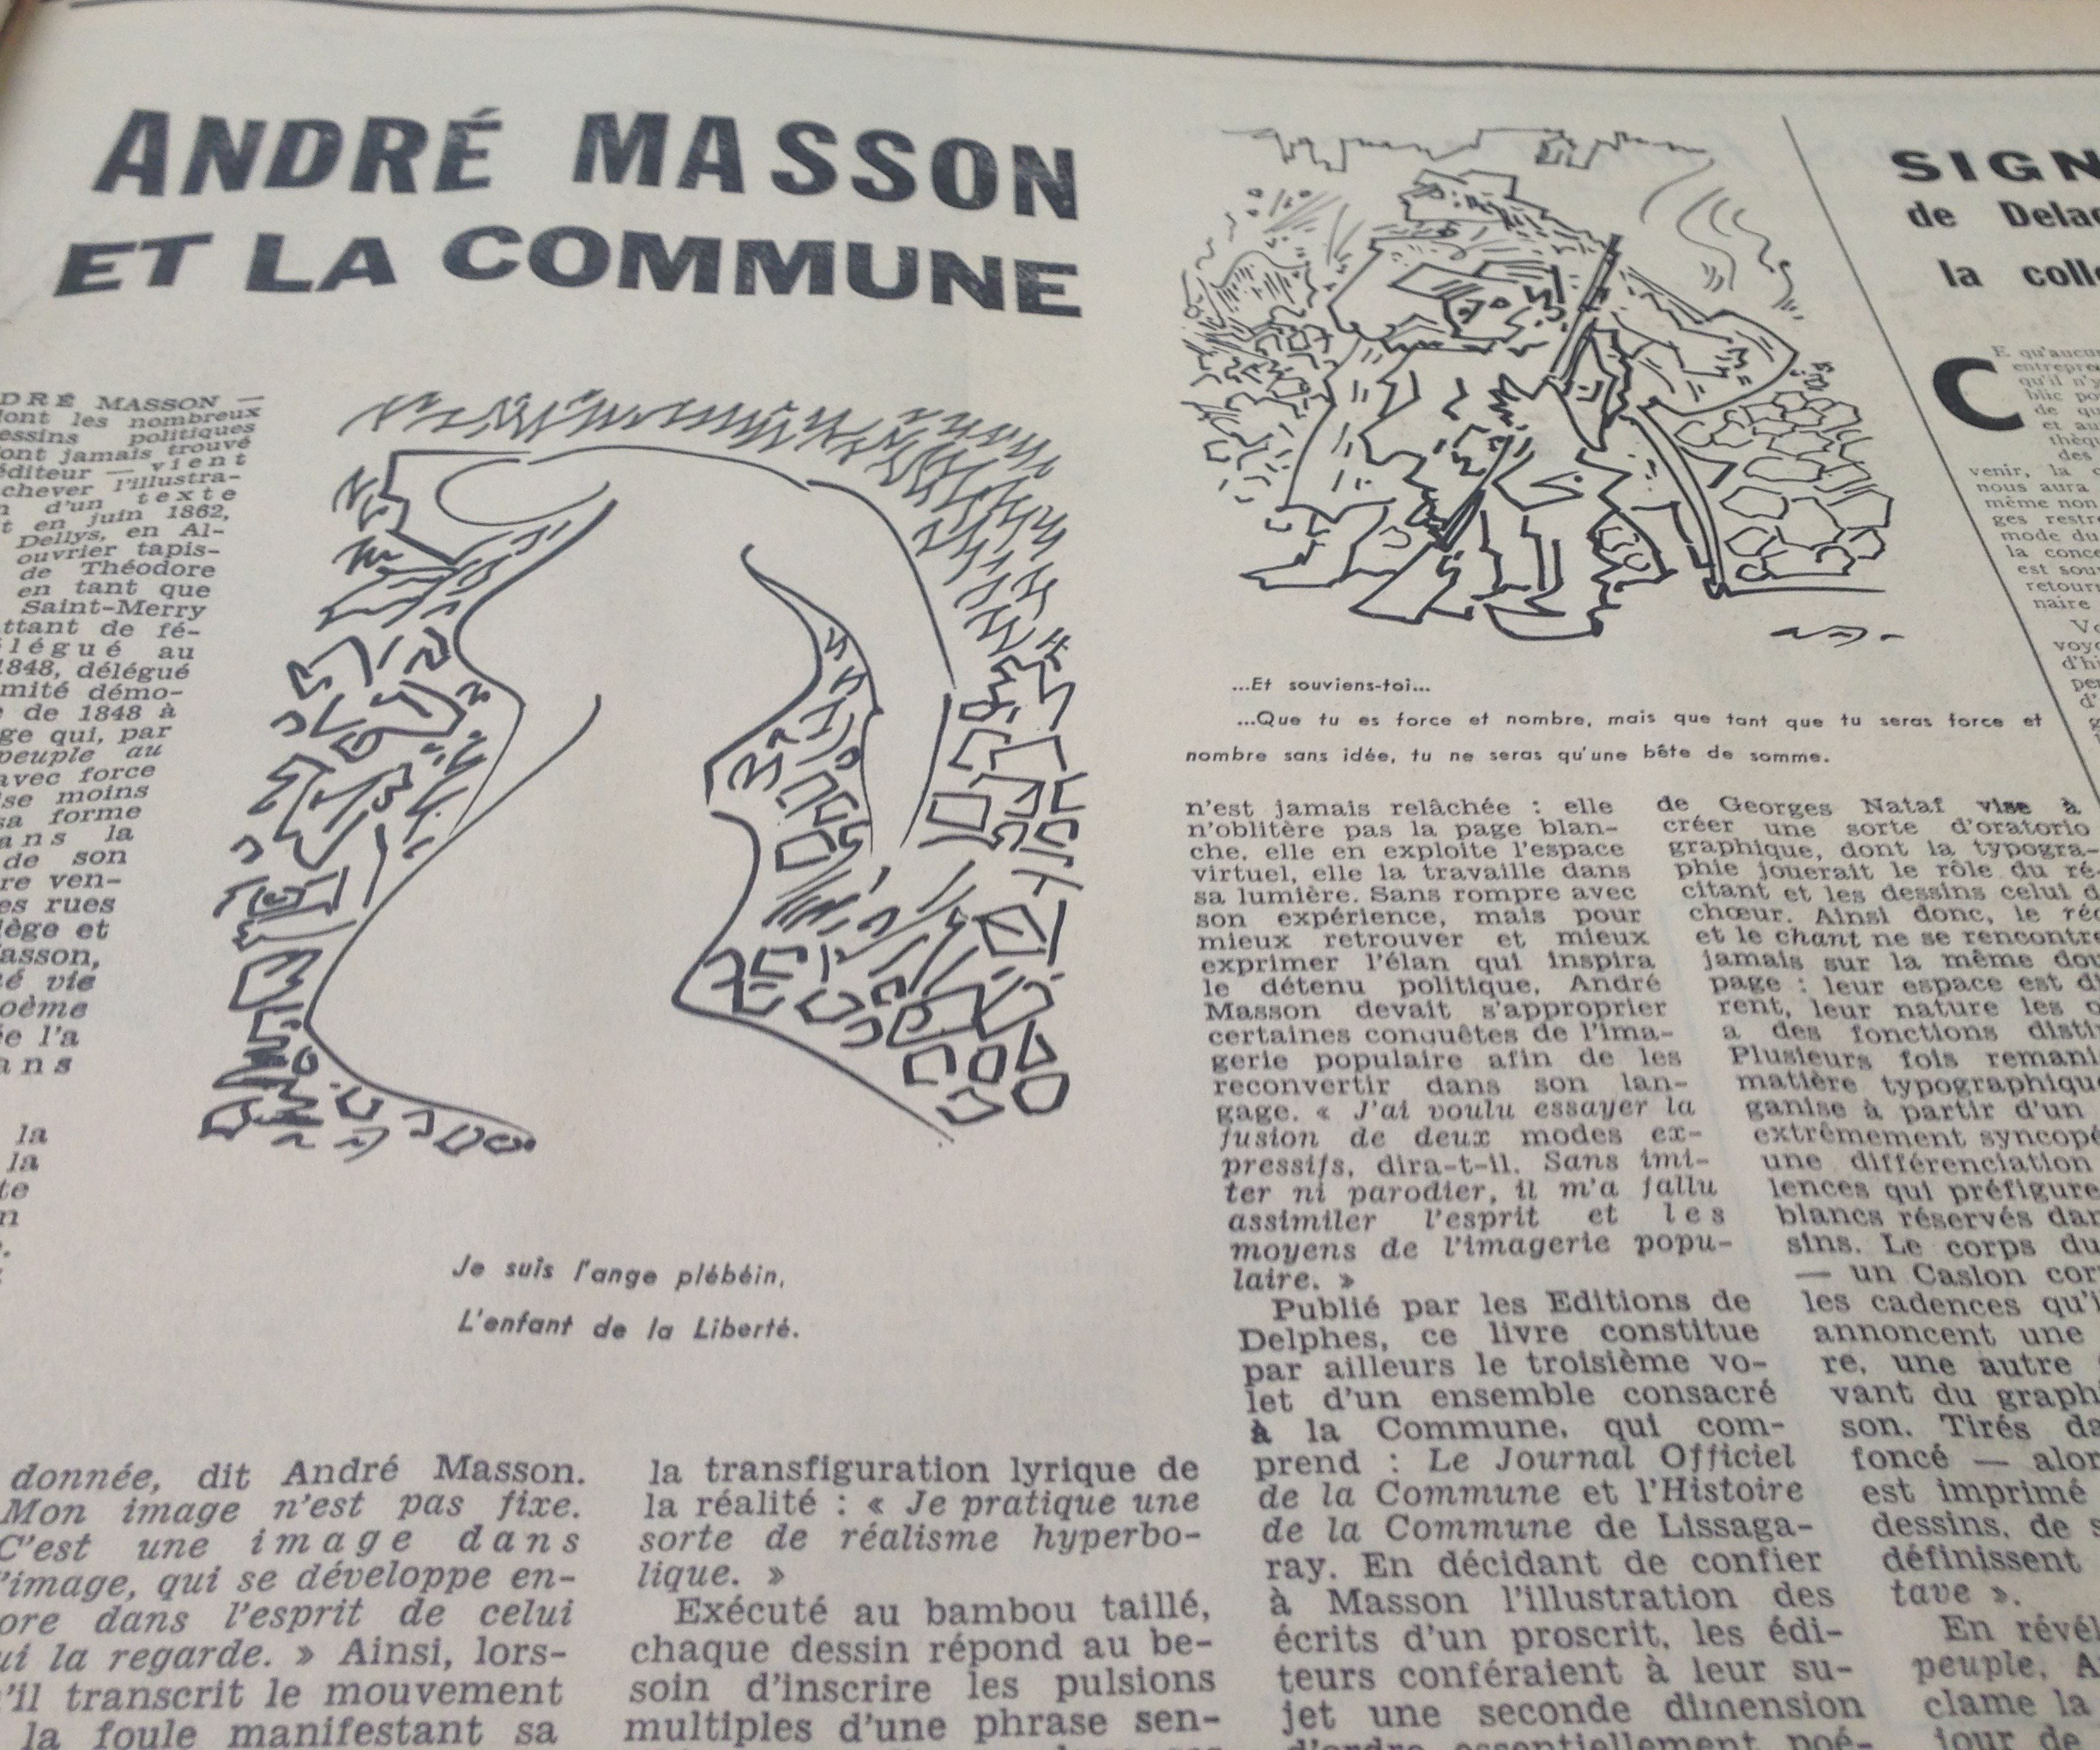
\includegraphics[width=0.33\textwidth]{massoncommune}
	\caption{\cite{commune}}\label{articlemoulin}
\end{figure}


 Antérieur à la fameuse période de la Commune de Paris de 1871 indiquée dans le titre, ce poème de 1862 est néanmoins placardé dans les rues de Paris pendant cette révolution populaire. A l’image de la condition sociale du poète dont Moulin rappelle le riche passé politique, avec notamment un Coup d’Etat qui lui a valu le bagne en Algérie durant la rédaction de ce poème, le critique d’art qualifie la « force » de ce dernier tirée d’une \enquote{franche simplicité du discours}. On retrouve dans le champ lexical du critique l’élan patriotique des Parisiens qui prennent le fusil pour défendre leur ville et leurs idéaux républicains face à l’armée versaillaise de Thiers et ses représentants monarchistes. Le critique clôt d’ailleurs ce paragraphe introductif de repère historique avec les propres mots du dessinateur et peintre André Masson sur son rapport à la Commune : \enquote{la Commune a donné vie à un authentique poème d’agitation.}

	  Ainsi, illustrer le poème \emph{Le peuple au peuple} reviendrait à considérer celui-ci comme le symbole de cette révolution populaire, dont lui donner image perpétuerait le mouvement insurrectionnel des Communards. On retrouve également le terme du recueil du \emph{Mouvement perpétuel} d’Aragon et la force subversive présupposée dans ce mouvement infini. Or, ce même mouvement, prêté par Masson à la Commune, est également celui qui \enquote{l’a constamment guidé dans son travail}. Ainsi, de même que \emph{Le peuple au peuple}, les oeuvres de Masson semblent puiser leur force dans l’élan, le mouvement pur, le mouvement comme signe. 

	Le second paragraphe insiste sur la pauvreté des témoignages des écrivains et des artistes au sujet de la Commune. Si, de la part des écrivains, cela peut s’expliquer par le fait qu’une majorité d’entre eux était hostile aux Communards, cela peut paraître plus étonnant du côté des artistes, puisque les semi-marginaux prenaient une part active aux événements aux côtés de la petite bourgeoisie (dans laquelle on retrouve Théodore Six). Même de la part d’un grand représentant tel que Courbet, à la tête de la fédération des artistes, Masson n’a connaissance que de \enquote{quelques croquis de Courbet et un ignoble livre de Gustave Courbet contre les Communalistes}. 

    Le choix d’illustrer cette révolution populaire montre donc la volonté du dessinateur de réhabiliter cette part de l’Histoire afin de la préserver du risque d’oubli. Mais la seconde moitié du paragraphe ouvre sur un second sujet plus riche de sources, celui du rôle des femmes sous la Commune : \enquote{En revanche, la première héroïne dont j’ai entendu parler dans mon enfance, ce n’était pas Jeanne d’Arc mais Louise Michel. Ma mère était une admiratrice passionnée de Louise Michel}. Avec cette référence, Masson se situe dans un geste de transmission, à l’image de celui de sa mère qui l’a directement sensibilisé à cette période historique. Il se fait par le biais maternel lui-même enfant d’une Louise Michel. Entre autres, en ce qui concerne le rôle actif des femmes, incarné par cette institutrice. On imagine ainsi la relation intime de Masson pour l’histoire de la Commune grâce à la transmission familiale des forts idéaux républicains de Louise Michel, mais peut-être aussi l’héritage de son geste transgressif. Si Masson est d’une génération qui n’a pas vécu la Commune, né une vingtaine d’années plus tard, l’imaginaire autour de cette révolution populaire se forme d’abord grâce au témoignage maternel, donc à la mémoire collective. 

    C’est pourquoi Moulin ouvre son troisième paragraphe sur le rapport de Masson à la femme : \enquote{La République est femme; elle enfante les hommes}. Ainsi, à l’image de Louise Michel, la femme incarne pour Masson le mouvement subversif qui défend ses idéaux. Le mythe autour de la \enquote{Vierge Rouge} est clairement revendiqué. Celle-ci dépasserait même l’égalité avec l’homme pour lui être supérieur, puisqu’elle l’\enquote{enfante}. Cette vision de la femme se rapproche de  la position de son ami Aragon. Pour autant, cette « fonction symbolique ne la prive pas de sa perspective réelle : elle tient sa place sur les barricades ou dans les ruines ». Or, c’est cette attitude révolutionnaire qui constitue pour Masson la beauté des femmes incarnée sous la Commune. A la fois membres du peuple et par leur geste patriotique de prendre le fusil à la Place Blanche pendant la Semaine Sanglante .


    Ainsi, la femme sous la Commune est comparée dans l’article de Moulin à l’idée de mouvement : \enquote{une même arabesque la décrit et l’environne, la liant à l’action dont elle émerge en armes}. Cette métaphore graphique du cycle montre la correspondance des idéologies défendues par ces femmes et leur mouvement insurrectionnel, ce qui justifie l’inspiration qu’elles procurent aux illustrations de Masson, où la forme exemplifie les idéaux. Ainsi, à partir de ce mouvement, Masson en retrouve d’autres analogues, tels « la guerre d’Espagne, ne voulant jamais suivre le texte à la lettre ni se laisser fermer dans l’anecdotique ». Cette autre guerre civile, de 1936 à 39, peut faire écho à la Commune sous divers points, notamment en raison des combats républicains contre les nationalistes. L’échec des républicains qui donne lieu à la dictature de Franco est d’autant plus emblématique puisque, cette fois, Moulin précise la présence de Masson durant la guerre, \enquote{si bien que toute figure dressée dans la lutte implique graphiquement tout un peuple}: L’unité du peuple est illustrée chez Masson par la représentation d’un de ses membres qui les symbolise tous. Au nom certainement d’une autre représentation de Masson, \enquote{l’ange Liberté} dont \emph{une blancheur inaltérable, préserve sa puissance mythique de la réalité qui l’assaille}. On comprend par cette pureté symbolique de la Liberté qu’il s’agit pour Masson d’une valeur universelle à défendre communément pour tous les peuples, époques et lieux confondus. 


Le journaliste Moulin illustre ainsi comment, à partir des idéaux défendus dans les illustrations du livre de Masson, la forme graphique prend forme et mouvement dans le dessin même. Masson évoque d’ailleurs une mise en abyme :\enquote{Mon image n’est pas fixe. C’est une image dans l’image, qui se développe encore dans l’esprit de celui qui la regarde}. Ainsi, le mouvement échapperait à son propre créateur selon celui qui le regarde, ce qui montre la volonté subversive des dessins : \enquote{Je pratique une sorte de réalisme hyperbolique}.Le fait que cette formule quasiment antithétique ne soit suivie d’aucune précision montre sa volonté de jouer sur une forme d’ambiguïté. On est plus proches de l’\enquote{art romanesque} selon Aragon que du réalisme balzacien.

	Au mouvement caractéristique des illustrations se reflète dans un effet-miroir sa technique, le \enquote{bambou taillé}, un type d’encre : \enquote{chaque dessin répond au besoin d’inscrire les pulsions multiples d’une phrase sensible, aussi diverse dans ses cassures que dans ses attaques}.Les dessins sont donc pour Masson un moyen d’exprimer fidèlement la force subversive du poème. Or, plutôt que d’une violence, c’est le lyrisme qui est réhabilité lorsque Moulin évoque une \enquote{tension mélodique}. Pourtant, ce lyrisme est réhabilité graphiquement par les illustrations, \enquote{pour mieux retrouver et mieux exprimer l’élan qui inspira le détenu politique}. 

Le lyrisme est donc bel et bien entremêlé à la dimension insurrectionnelle du poème. C’est ce même croisement qui inspire les dessins dans un souci de fidélité à l’esprit du poème, et à travers de l’esprit de révolution populaire. A la violence présupposée, la beauté insurrectionnelle s’exprime au contraire par le lyrisme, \enquote{sans imiter ni parodier, il m’a fallu assimiler l’esprit et les moyens de l’imagerie populaire}: Si l’expression graphique de Masson témoigne de sa vision personnelle des événements, c’est aussi par souci de réhabilitation du regard sur les événements, où il s’agit de leur donner vie. Mais cette réhabilitation demande néanmoins selon le dessinateur de passer par une connaissance autant des états d’esprits de l’époque que de leurs images, à partir desquels seulement l’artiste livre son regard mouvant. 

%Mettre illustrations de Masson 

Par ailleurs, puisqu’il s’agit d’un troisième volet dédié à la Commune, Moulin précise la dimension poétique du livre prodigué par les illustrations de Masson, en plus de l’historicité des événements. La dimension lyrique se retrouve dans la mise en page de Nataf, disposée comme une chorale, \enquote{une sorte d’oratorio graphique, dont la typographie jouerait le rôle du récitant et les dessins celui du choeur}. Cette division permet d’introduire une rythmique de l’espace, entre la typographie et le blanc de la page. Moulin évoque même \enquote{le corps du caractère — un Caslon corps 20— et les cadences qu’il détermine annoncent une autre lecture, une autre couleur dérivant du graphisme de Masson}. Ainsi, on peut apercevoir dans la forte présence musicale tant dans les dessins que la mise en page une évocation lyrique de la Commune comme l’incarne compositeur Jean-Baptiste Clément. 

L’image d'\enquote{une autre octave} semble chercher à retrouver sur le papier la musicalité du compositeur de la Commune. De même, l’allusion appuyée par l’italique de la \emph{couleur} induite dans les dessins de Masson semble figurer symboliquement le \enquote{rouge cerise} emblématique du lyrisme de l’histoire de la Commune. Le choix du lyrisme à part entière est donc déterminant dans cette lecture voulue poétique de l’histoire de la Commune. Face à la violence très marquée, notamment par les exécutions des Communards par l’armée versaillaise lors de la Semaine Sanglante, lui est opposé le lyrisme insurrectionnel. Le réhabiliter, comme le souligne en conclusion Raoul-Jean Moulin, c’est aussi raviver cette valeur lyrique dans cette révolution populaire, et plus globalement d’un mouvement révolutionnaire face à toute forme d’oppression. 

Pour exemplifier la critique de Moulin, deux dessins de Masson avec des légendes tirées du poème encadrent les paragraphes.  Le dessin de gauche illustre des vers dans la partie \emph{Le rêve du poème}, \enquote{Je suis l’ange plébéien / L’enfant de la Liberté}. On reconnait grâce à la légende le fameux ange de la Liberté évoqué par Moulin. Le dessin illustre un corps aux multiples courbes. Plutôt que dans les airs, l’ange en question semble allongé dans un univers réaliste : on identifie la forme des touffes d’herbes et la forme de feuilles d’arbres. L’ange n’a d’ailleurs pas d’ailes, et sa tête sans visage a le cou courbé dans l’herbe. La courbe de son corps,le trait inachevé de la tête et les lignes des doigts se complètent avec les brindilles d’herbes et de feuilles. Ainsi, cet ange comme symbole du peuple fait corps avec la nature dans une parfaite harmonie. Au lieu d’arrêter le mouvement de la nature, les traits du corps semblent suivre leur élan, tout en étant dans une attitude de repose qui montre sa tranquillité d’esprit.

% Image : Dessin de l'article 

Le poème aligné en haut à droite de l’article illustre la partie  \emph{Remember!} du poème, avec pour légende :\enquote{…Et souviens-toi…/…Que tu es force et nombre, mais que tant que tu seras force et / nombre sans idée, tu ne seras qu’une bête de somme}. Ces vers à valeur de maxime pouvaient à l’époque de la Commune paraître comme une main tendue vers les Provinciaux. Ces derniers s’opposaient à la Commune en se réclamant de la paix. Seulement, dans l’esprit des Communards, il s’agissait en réalité de défendre les mêmes idéaux de classes modestes qui combattent pour leur terre et le travail.

Ce lyrisme patriotique est illustré par Masson avec deux protagonistes au coeur du dessin. Celui debout à la gauche du lecteur semble porter un chapeau de paille et des vêtements modestes. A ses côtés, un personnage agenouillé avec une casquette, des bottes et des épaulettes tient un fusil. On peut y voir ainsi la représentation du paysan à côté du soldat. La cause de l’homme de la terre et celui de la ville, peut-être un représentant de la garde nationale, est unifiée. A l’arrière plan, on trouve une ligne de bâtiments qui évoque des barricades. Deux chemins y mènent respectivement, l’un partant du côté du paysan, l’autre de celui du soldat. Bien que le mouvement des traits paraisse plus discernable que les formes représentées, on reconnaît la forme des pavés qui mènent jusqu’aux barricades.
%image n2

 Malgré le mouvement du décor avec un chemin ponctué par de multiples traits, les deux personnages semblent attendre : Le paysan a les bras croisés et le soldat ne se sert pas de son fusil pour tirer, même si sa position le représentent en alerte dans une attitude de défense. Sur le chemin de gauche, une forme de rechange courbée semble représenter un visage de femme. Sa tête en forme de drapeau rassemble autour d’elle de multiples traits, ainsi qu’à l’intérieur du drapeau, et des envols de petits cailloux au-dessus de sa tête. Mais le côté droit du drapeau n’est pas complètement fermé. Ainsi, cette femme-drapeau semble s’adresser directement aux deux personnages. On peut y reconnaître la représentation de la République en femme caractéristique de Masson. C’est pourquoi les deux personnages unis, la distinction des traits de leurs corps respectifs est peu discernable, affichent une attitude plus de défense que d’attaque. Leur comportement protecteur pour le soldat et songeur pour le paysan illustre la légende basée sur l’importance du mouvement perpétuel de la pensée du peuple. 

 Le croisement dans cet article de Raoul-Jean Moulin des témoignages intimes de Masson vis-à-vis de la Commune et de ses esquisses révèle quelle valeur éducative a été dans sa philosophie et son esthétique un tel événement. Puisque la Commune, que l’on soit du côté des Parisiens ou des Versaillais et Provinciaux est ressentie comme la libération la plus totale du peuple, y compris au sens du libertinage avec le retour du peuple à ses instincts primaires. Valorisé par les communards ou condamnés après la Commune par ses ennemis, la libération des corps et des moeurs est son élément particulier qui la distingue des autres insurrections. C’est pourquoi la Commune ne peut que naturellement s’imbriquer dans l’idéologie de Masson, et l’on sait combien le mot « révolution » revient fréquemment comme martelé dans ses correspondances, et que celle-ci est aussi proprement physique. C’est donc aussi une influence proprement esthétique que joue sur André Masson un exemple de liberté absolue des expressions du peuple auquel Masson choisit clairement de se confondre. 

\subsection{La sensiblité communarde d'Aragon}

Relever l'affect commun chez Aragon comme chez Masson autour de la Commune de Paris manifeste une fois à la fois une proximité et une profonde distinction. Cette distinction serait probablement à situer à la mémoire histoirique après la Commune, c'est-à-dire à l'adhésion d'Aragon au Parti Communiste et aux réserves de Masson sur les théories marxistes. Autrement dit, la sensibilité d'Aragon vis-à)vis de la Commune de Paris se situe dans l'héritage de l'histoire du communisme, et, plus particulièremet, à la conception de la Commune comme l'événement qui engendrera la Révolution Russe d'Octobre 1917, rêve déjà présent dans les esprits des révoltuionnaires de 1917 : 

\begin{quote}
\emph{On sait que le révolutionnaire russe avait dansé dans la neige lorsque la durée du pouvoir des soviets eut dépassé de vingt-quatre heures seulement celle de la Commune de Paris, et qu’il dort, dans son mausolée, enveloppé du drapeau de l’un des bataillons de la garde nationale insurgée en 1871. Pour Staline encore, qui ici paraphrase Marx :} « La République des Soviets est la forme politique recherchée et enfin trouvée, dans le cadre de laquelle doit être réalisée l’émancipation économique du prolétariat, la victoire complète du  socialisme. La Commune de Paris a été l’embryon de cette forme. Le pouvoir des Soviets en est le développement et le couronnement.\footcite[p241]{proces}\end{quote}

La valeur défendue par Aragon du réalisme socialiste prend ainsi en compte à la fois l'héritage de la Commmune de Paris comme première pierre de l'édifice communiste, c'est-à-dire que le \enquote{réalisme socialiste} ne peut exister également qu'à partir de la Commune de Paris. Cette référence histoirique lui permet d'ailleurs de propager à la fois le réalisme socialiste et légitimer l'idéologie communiste en France : 

\begin{quote}
“Non, le type soviétique d’Etat n’est pas spécifiquement russe. Il est né de la Commune de Paris: il n’a pu se développer que grâce à l’expérience de la lutte de classe internationale, dont les bolcheviks ont su tirer les leçons. Mais dans son application dans l’U.R.S.S. même, il faut toute l’ignorance volontaire de nos démocrates bourgeois pour prétendre qu’il s’agit là d’une expérience spécifiquement russe.“\footcite[p121]{lavoinne}	
\end{quote}

Néanmoins, cet imaginaire romantique autour de la Commune est représenté dans l'esprit d'Aragon par la figure de Rimbaud. Ce choix n'est pas anodin, d'autant plus que, avec Lautrémont, Rimbaud avait été l'un des sujets d'affinités entre les jeunes médecins Aragon et Breton rencontrés sur le Front. Tout comme Rimbad figure parmi les grands noms dont se revendiquent le groupe surréaliste. Il est donc intéressant que Rimbaud accompagne Aragon tant à l'aube de la période dada, pendant l'époque surréaliste, et durant son engagement politique : \enquote{Aragon liera au nom de Rimbaud l’image de la révolte et du peuple insurgé de la Commune de Paris, et il retrouvera bientôt chez un grand nombre de peintres français le réalisme qu’il admire chez Cézanne et Courbet.}\footcite[p165]{these}

Aragon se passionnerait-il pour la Commune à partir de sa fascination première pour Rimbaud ? Toujours est-il que sa présence, comme celle de la Commune, attribuent une certaine forme subervise envisagée dans la vision du réalisme socialiste, en ce sens où le réalisme socialiste, en se positionnant du côté du peuple, se comporterait par nature comme un mouvement révolutionnaire :

\begin{quote}
Aragon explique (ibid., p. 241) :\enquote{On doit se souvenir de ce fait très simple qu’Arthur Rimbaud en 1871 était venu tout naturellement à Paris s’engager dans l’armée de la Commune. Ses poèmes de cette époque sont des poèmes à la gloire de la Commune. Que serait-il advenu de Rimbaud dans une Commune triomphante ? Nous l’ignorons, mais nous savons ce qu’il en est advenu, la Commune vaincue} : telle est l’interprétation marxiste de son fameux \enquote{silence}, une interprétation de plus.\footcite[p241]{these}	
\end{quote} 

En entremêlant la destinée de Rimbaud et celle de la Commune à la fin de celle-ci, Aragon livre un symbole fort : le poète, c'est-à-dire l'écrivain selon la conception réalsite socialiste, se situe parmi les membres du peuple dans le cycle révolutionnaire et son existence en tant que poète est ancrée dans celle du mouvement qui le soulève. C'est pourquoi le réalisme socialiste, même si au premier abord l'idée peut paraître contradictoire avec la notion \enquote{réaliste} doit se concevoir doit une atmosphère de lyrisme révolutionnaire. 

En outre, on peut soupçonner que le rapport d'Aragon vis-à-vis de la Commune, et peut-être plus encore comme le montre l'exemple de Rimbaud la proximité avec l'échec de la Commune, dépasse la thèse communiste et agit aussi comme un repérage historique dans un niveu plus intime : Dans \emph{Les voyageurs de l'Impériale}, le personnage principal, le grand-père Pierre Mercadier était présent pendant la Commune : 
\begin{quote}
 Il redoutait les aléas de l’avenir du monde. Il avait traversé des bouleversements, il savait au fond la fragilité de l’édifice social. Né en 1856, il avait passé son enfance dans le temps de l’Empire libéral. […] L’Empire était tombé, les Prussiens campaient un peu partout en France, il y avait eu la Commune, et Pierre Mercadier n’avait encore que quinze ans.\footcite[p43]{voyageursdelimperiale}\end{quote}

 Comme Rimbaud, le personnage Pierre Mercadier inspiré en partie par le grand-père maternel d'Aragon a neuf années de moins que la personne réelle Fernand de Biglione, de telle sorte qu'il vit la Commune adolescent et non pas adulte. Cette réflexion illustre l'atmoshpère romantique qu'Aragon se fait de la Commune, conçue pour être vécue par son peronnage en pleine période d'émancipation, à un moment où la défaite de la Commune a un impact fodnateur dans cette période de transition qu'est l'adolescence. 

 Plus généralement, dans \emph{Les Voaygeurs de l'Impériale}, l'échec de la Commune agit comme un spectre, c'est-à-dire qu'elle agit comme un traumatisme pour les personnages les plus âgés du romans, tels que Pierre Mercadier ou l'oncle Blaise :

 \begin{quote}
 La France sortait d’un cauchemar prolongé. Les hommes nés pendant la guerre allaient avoir trente ans. Ainsi l’on atteignait graduellement à l’oubli de l’invasion. Le souvenir des luttes intestines demeurait plus vivace parce qu’à la Commune avaient succédé les bannissements, les ostracismes, parce que de la Commune était née une grande peur qui ne faiblissait pas au coeur de  ceux qui l’avaient tuée.\footcite[p459]{voyageursdelimperiale}\end{quote}

 Avec cette présence discrète mais persistante de la Commune à l'image d'un spectre dans tout le roman, Aragon dévoile ici une conviction à partir de l'échec de la Commune, qui serait celle d'une résurrection possible pour celle-ci, c'est-à-dire une revanche à prendre,celle du prolétariat sur la bourgeoisie. De telle sorte que la temporalité du roman est encadrée entre la défaite de la Commune et la veille de la 1ère Guerre Mondiale. Or, cette vision temporelle ne s'explique pas uniquement d'après la perespctive du réalisme socialiste, puisque l'on retrouve ces deux références historiques dans \emph{Blanche ou l'oubli}:

 \begin{quote}
Entre cet été pluvieux où Marie Noire sur la Côte mesure au peu d’entrain de son ami saisonnier que la jeunesse porte en elle sa fin et ces après-midi avenue Victor-Hugo chez Maryse, il y a le temps qui sépare la Commune de Paris de l’éclatement de la guerre en 14. Je me fais l’effet d’une vieille pendule qui ne s’est pas contentée de la durée des autres. Est-ce qu’en 1914 j’avais la moindre représentation de la vie à Paris en 71 ? Pourquoi le joueur de volley-ball devrait-il se faire une image exacte du Mouvement Dada ? ou du salon de l’avenue Victor-Hugo ?\footcite[p38]{blancheouloubli}\end{quote} 

Ainsi, la Commune n'est pas seulement un repère temporel, puisque, ancrée dans l'obsession plus génrale du temps chez Aragon dans ses oeuvres, la Commune est vue comme un élément romanesque. C'est d'ailleurs la transition du temps de la Commune qui semble fasciner Aragon: La défaite de la Commune, c'est-à-dire l'après les événements de la Semaine Sanglante, la transition. Mais la figure du Rimbaud adolescent comme celle de Pierre Mercadier conçoit la Commune vécue dans l'imaginaire romantique comme une période de transition, entre deux âges. Dans la conception romanesque d'Aragon et son rapport au temps, la Commune est un élément d'entre-deux. 
 
\subsection{La référence prépondérante de la Commune dans l'Histoire des \emph{Lettres françaises}}

En outre, si la Commune joue un rôle dans la conception idéologique et comme marqueur temporel dans l'oeuvre d'Aragon, elle influence également son parcours journalistique, dans la lignée de celui de membre du Parti Communiste. Sans En 1934, Aragon militant est rédacteur à la fois dans le journal \emph{L'Humanité} et dans la revue \emph{Commune}, pour laquelle Aragon est rédacteur pour la rubrique \emph{Les Livres}. En plus d'un titre à la référence transparente, la revue est dirigée en partie par Paul Vaillant-Couturier au nom de l'A.E.A.R (Association Des Ecrivains Révolutionnaires).\enquote{La Commun}e sert donc à mentionner l'idéologie communiste, en particulier à fixer la valeur révolutionnaire comme exigence de son discours.Le propre discours d'Aragon emprunte des voies différentes en fonction du type de public différent socialement pour qualifier le réalisme socialiste qu'il cherche à propager en France : 

\begin{quote}
 Sur le plan journalistique d’autre part on notera que \emph{Commune}, revue pour les intellectuels, utilise plus volontiers que \emph{L’Humanité} l’expression “réalisme socialiste“. Mais entre la revue et le quotidien, une identique volonté de lier politique et littérature conduit à une large communauté de vues.\footcite[p157]{lavoinne}\end{quote}

Ainsi, même en prenant en considération une éventuelle réception distincte de deux type de lecteurs, Aragon vise avant tout un choix de politique éditoriale qui n'est pas sans rappeler celui à venir des \emph{Lettres françaises} : bien qu'il s'agisse avant tout d'un journal culturel,le propos politique est ancré dans la critique. Ce choix de conciliation n'est pas anodin, il correspond à une philosophie, peut-être d'ailleurs malgré des voies différentes à long terme proche d'André Masson, puisque, comme ce dernier, Aragon la qualifie de \enquote{vie} :

\begin{quote}
 L’activité du public lui apparaissait comme le plus sûr gage d’amélioration d’une revue qui “n’est pas sans défauts: ses numéros n’ont pas toujours l’équilibre souhaitable, et ce n’est que récemment,  et d’ailleurs sous le feu de la critique de son public, qu’elle a su vraiment organiser sa partie la plus vivante, ses chroniques qui vont de l'actualité des livres, du cinéma à celle des journaux et de la rue, de la vie même.“ On notera ici que l’ancien surréaliste et le journaliste s’alliaient chez Aragon pour faire sortir une revue intellectuelle des sentiers battus du débat théorique pour flairer le vent de l’éventuel, humer l’air du temps au-delà des frontières de l’imprimé.\footcite[p205]{lavoinne}\end{quote}

Ces quelques lignes laissent déjà pressentir son projet éditorial pour \emph{Les Lettres françaises} lorsqu'il en prend finalement la direction en 1953. On remarque d'ailleurs que, au service de la revue, l'imaginaire communard ne joue pas sur les mêmes aspects que dans les romans. De telle sorte que, au contraire de la défaite, Aragon cherche justement à redonner vie à l'esprit communard aussi bien dans \emph{Commune} que dans \emph{L'Humanité}:  

\begin{quote}
 Avant de tenter d’expliquer le comportement d’Aragon, il est nécessaire de compléter le tableau qu’il brossait de l’Union soviétique. En 1935, à son retour en France, il la célébra à l’occasion du 64ème anniversaire de la Commune de Paris dans une page spéciale de L’Humanité (17 mars 1935) : \enquote{Vive la Commune}. 
Le thème de la Commune permettait de réaffirmer le lien privilégié entre les prolétaires français et soviétiques. Comme tous les théoriciens marxistes, Aragon souligne en effet la relation entre l’insurrection parisienne de 1871 et la Révolution d’Octobre.\footcite[p133]{lavoinne}
\end{quote}

Ressuciter la Commune par un titre d'article voulu comme un cri,illustre le projet politique plus global d'Aragon et plsu généralement d'l'A.E.A.R. de renverser les valeurs bourgeoises par les idéaux révolutionnaires, en particulier en ce qui concerne les écrivains. Que cette commémoration paraisse dans \emph{L'Humanité,} un journal plutôt adressé aux ouvrirers induit à l'occasion de cet anniversaire que non seulement le Parti Communiste se fait leur représentant, mais surtout qu'il ambitionne de leur réattribuer l'esprit communard. Le modèle révolutionnaire tel que le conçoivent Aragon et Paul Vaillant-Couturier derrière l'A.E.A.R. 

Cette pratique des anniversaires, d'évenements forts ou de grands noms culturels et politiques, demeurera dans \emph{Les Lettres françaises} une marque de fabrique,avant la direction d'Aragon, mais peut-être plus souvent encore sous celle-ci. La Commune est parmi les anniversaires récurrents, et, dans les dernières années de la direction de Claude Morgan, lorsqu'Aragon dirige en novembre 1951 la nouvelle rubrique \emph{Tous les Arts}, en pleine année d'anniversaire de la Commune, la commémoration est poursuivie, après d'importantes pages publiées auparavant en mars et en mai jusqu'à en faire des sources documentaires conséquentes. Le directeur de l'époque, Claude Morgan s'inscrit dans un rapport à l'insurrection plus proche de la Révolution Française en convoquant la figure du révolutionnaire et proche de Robespierre Saint-Just :

\begin{quote}
Claude Morgan se référait à Saint-Just (dans son article du 9 septembre 1944) pour condamner toute indulgence ; un an plus tard, il use du même langage pour dénoncer \enquote{l'esprit de trêve} et exhorter \enquote{les honnêtes gens} à \enquote{reprendre celui du combat} en s'opposant à la \enquote{conjuration} des modérés : \enquote{chaque assassin gracié est un coup en pleine poitrine de l'innocent [...] un pas de plus et vous pouvez ouvrir la porte à Montherlant, à Giono.}\footcite[p538]{these}	
\end{quote}

\begin{figure}[H]
   \centering
   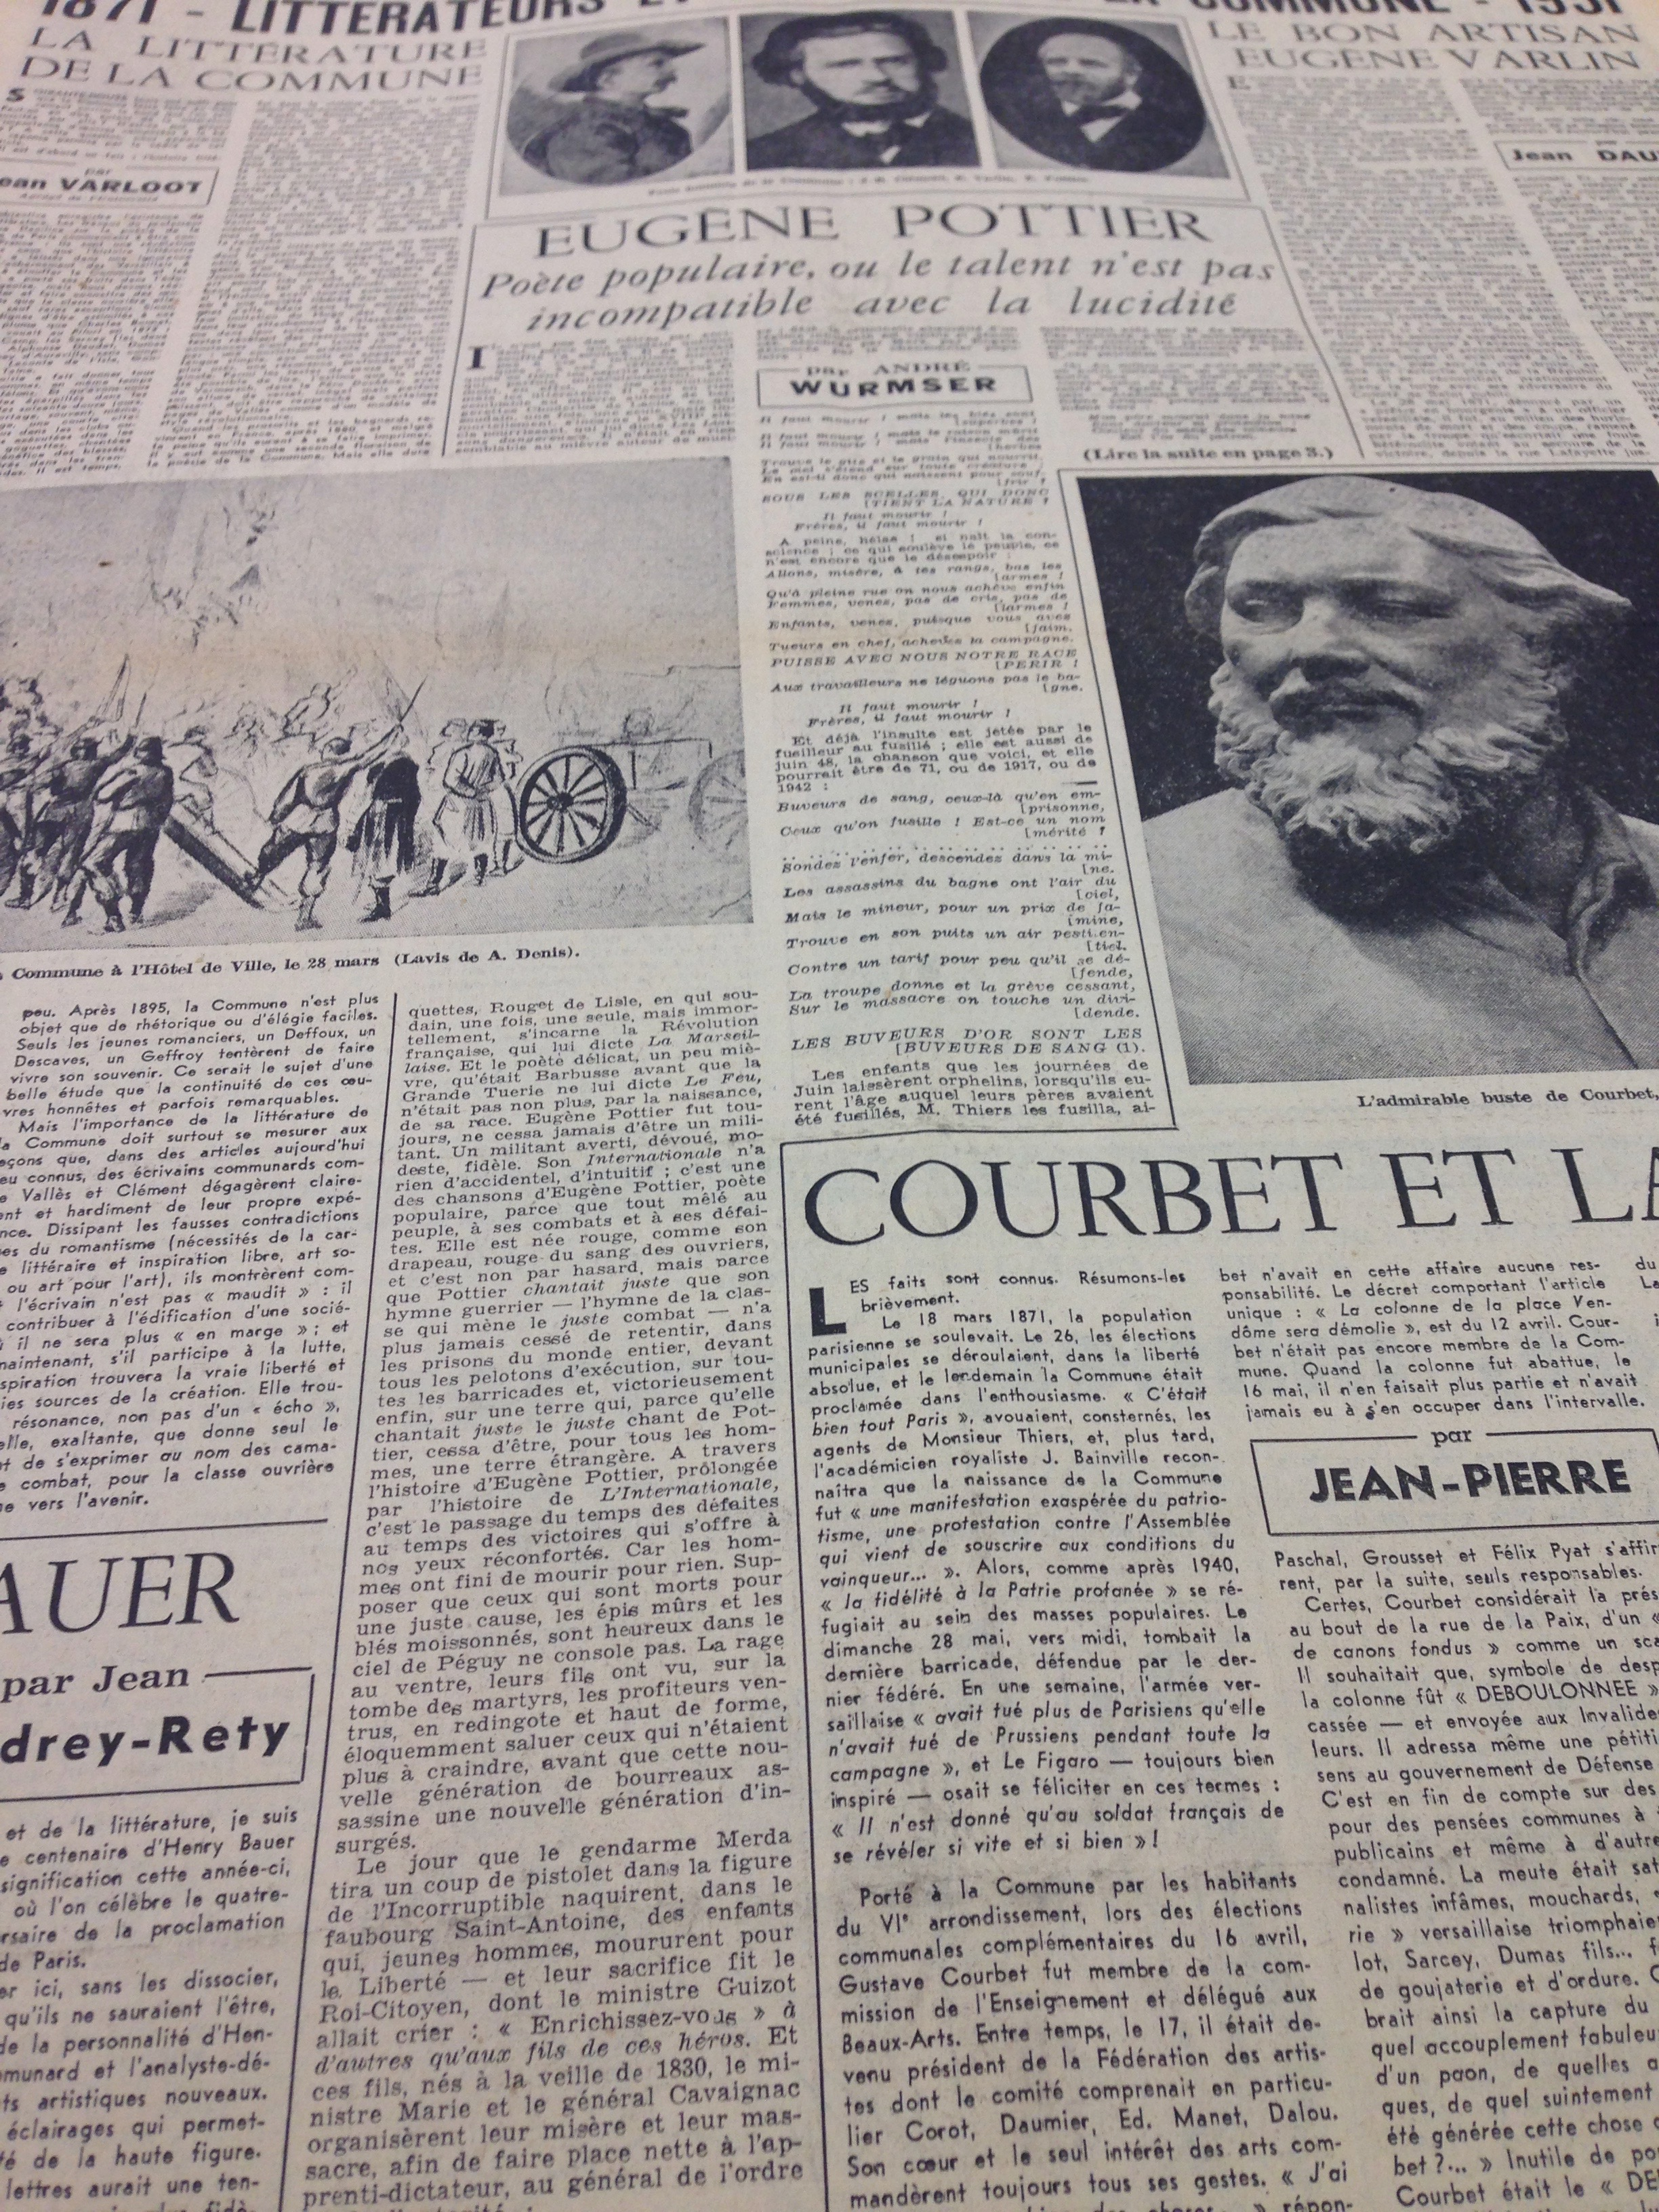
\includegraphics[width=0.33\textwidth]{courbetcommune}
	\caption{\cite{courbetcommunard}}\label{courbetcommune}
\end{figure}

Ainsi, même dix ans après son article de 1944, un mouvement insurrectionnel tel que la Commune ne sert pas exactement le même projet poltique que celle du renversement des valeurs idéolgiques au temps de \emph{Commune} et \emph{L'Humanité} dans les années 34-36. Or, un journal comme \emph{Les Lettres françaises} né sous la clandestinité de la résistance, fait de la Résistance à la fois son héritage et son mot d'ordre politique. Ainsi, les quatre-vingt ans de la Commune en 1951 servent un modèle de résistance, c'est-à-dire dans un sens plus large que celui de la défense de la cause ouvrière. Dans le premier article qu'il écrit dans la rubrique \emph{Tous les Arts} en novembre 51, Aragon publie un texte conséquent, \emph{Peindre a cessé d'être un jeu} dans lequel l'exemple de Courbet commuanrd sert d'exemple de peintre voué à la cause du \enquote{sentiment national}. Aragon écrit cet article en faisant référence à un fait d'actualité arrivé au Salon d'automne, pendant lequel sept tableaux du vernissage,sont retirés de l'exposition au moment de la visite présidentielle avec pour justification le \enquote{sentiment national}. Aragon, scandalisé par l'aspect \enquote{arbitraire} caché derrière le noble sentiment revient sur de grandes époques et de grands noms de la peinture à travers les siècles pour donner son conception du \enquote{sentiment national} : 
 
\begin{quote}
Quant à Courbet, ah! Courbet, un homme injurié, honni, condamné, traqué, exilé...Bien sûr, les Baylot d'alors ne l'aimaient pas, mais il fallut lui inventer l'histoire de la colonne Vendôme pour lui faire son affaire.[…] Les jeunes gens, même adonnés aux expériences les plus folles, aux rêves de la couleur et du trait, auront, désormais, devant les yeux, cet interdit du mensonge, comme aux jours de Vichy, quand nous écrivions, à chaque abandon au délire, à chaque mot risqué, nous nous rappelions ce qui était le feu véritable, et les héros dans les prisons et devant les pelotons d'exécution, les mots s'ordonnaient, suivaient un penchant tout autre, se gorgeaient du réel, du \emph{sentiment national}. 	
\end{quote}

Ainsi, la référence à l'un des plus épisodes de la Commune autour de la Colonne détruite alors que Courbet présidait la Fédération des Artistes, Aragon conteste d'abord la responsabilité de Courbet dans cette affaire, mais surtout il réhabilite l'image du peintre qui résiste en s'engageant dans la Garde Nationale pour défendre la ville de Paris. C'est donc une autre persective qu'Aragon aborde vis-à-vis de la Commune, celle de la défense à la fois de la ville et des causes idélogiques en train de germer au sein des classes parisiennes modestes. Mais la lutte des classes n'est plus tant la question, puisque l'image du peintre Courbet défendant les barricades est avant tout une image de liberté, probablement l'autre terme qui se cache derrière le mot d'ordre de Résistance. 



\section{De la Commune à la Résistance, ligne directrice des Lettres françaises (Illustration du tableau Résistance de Masson du numéro à côté du Sommaire}

\subsection{André Masson, médiateur entre Elsa Triolet et la Résistance}

\begin{figure}[H]
   \centering
   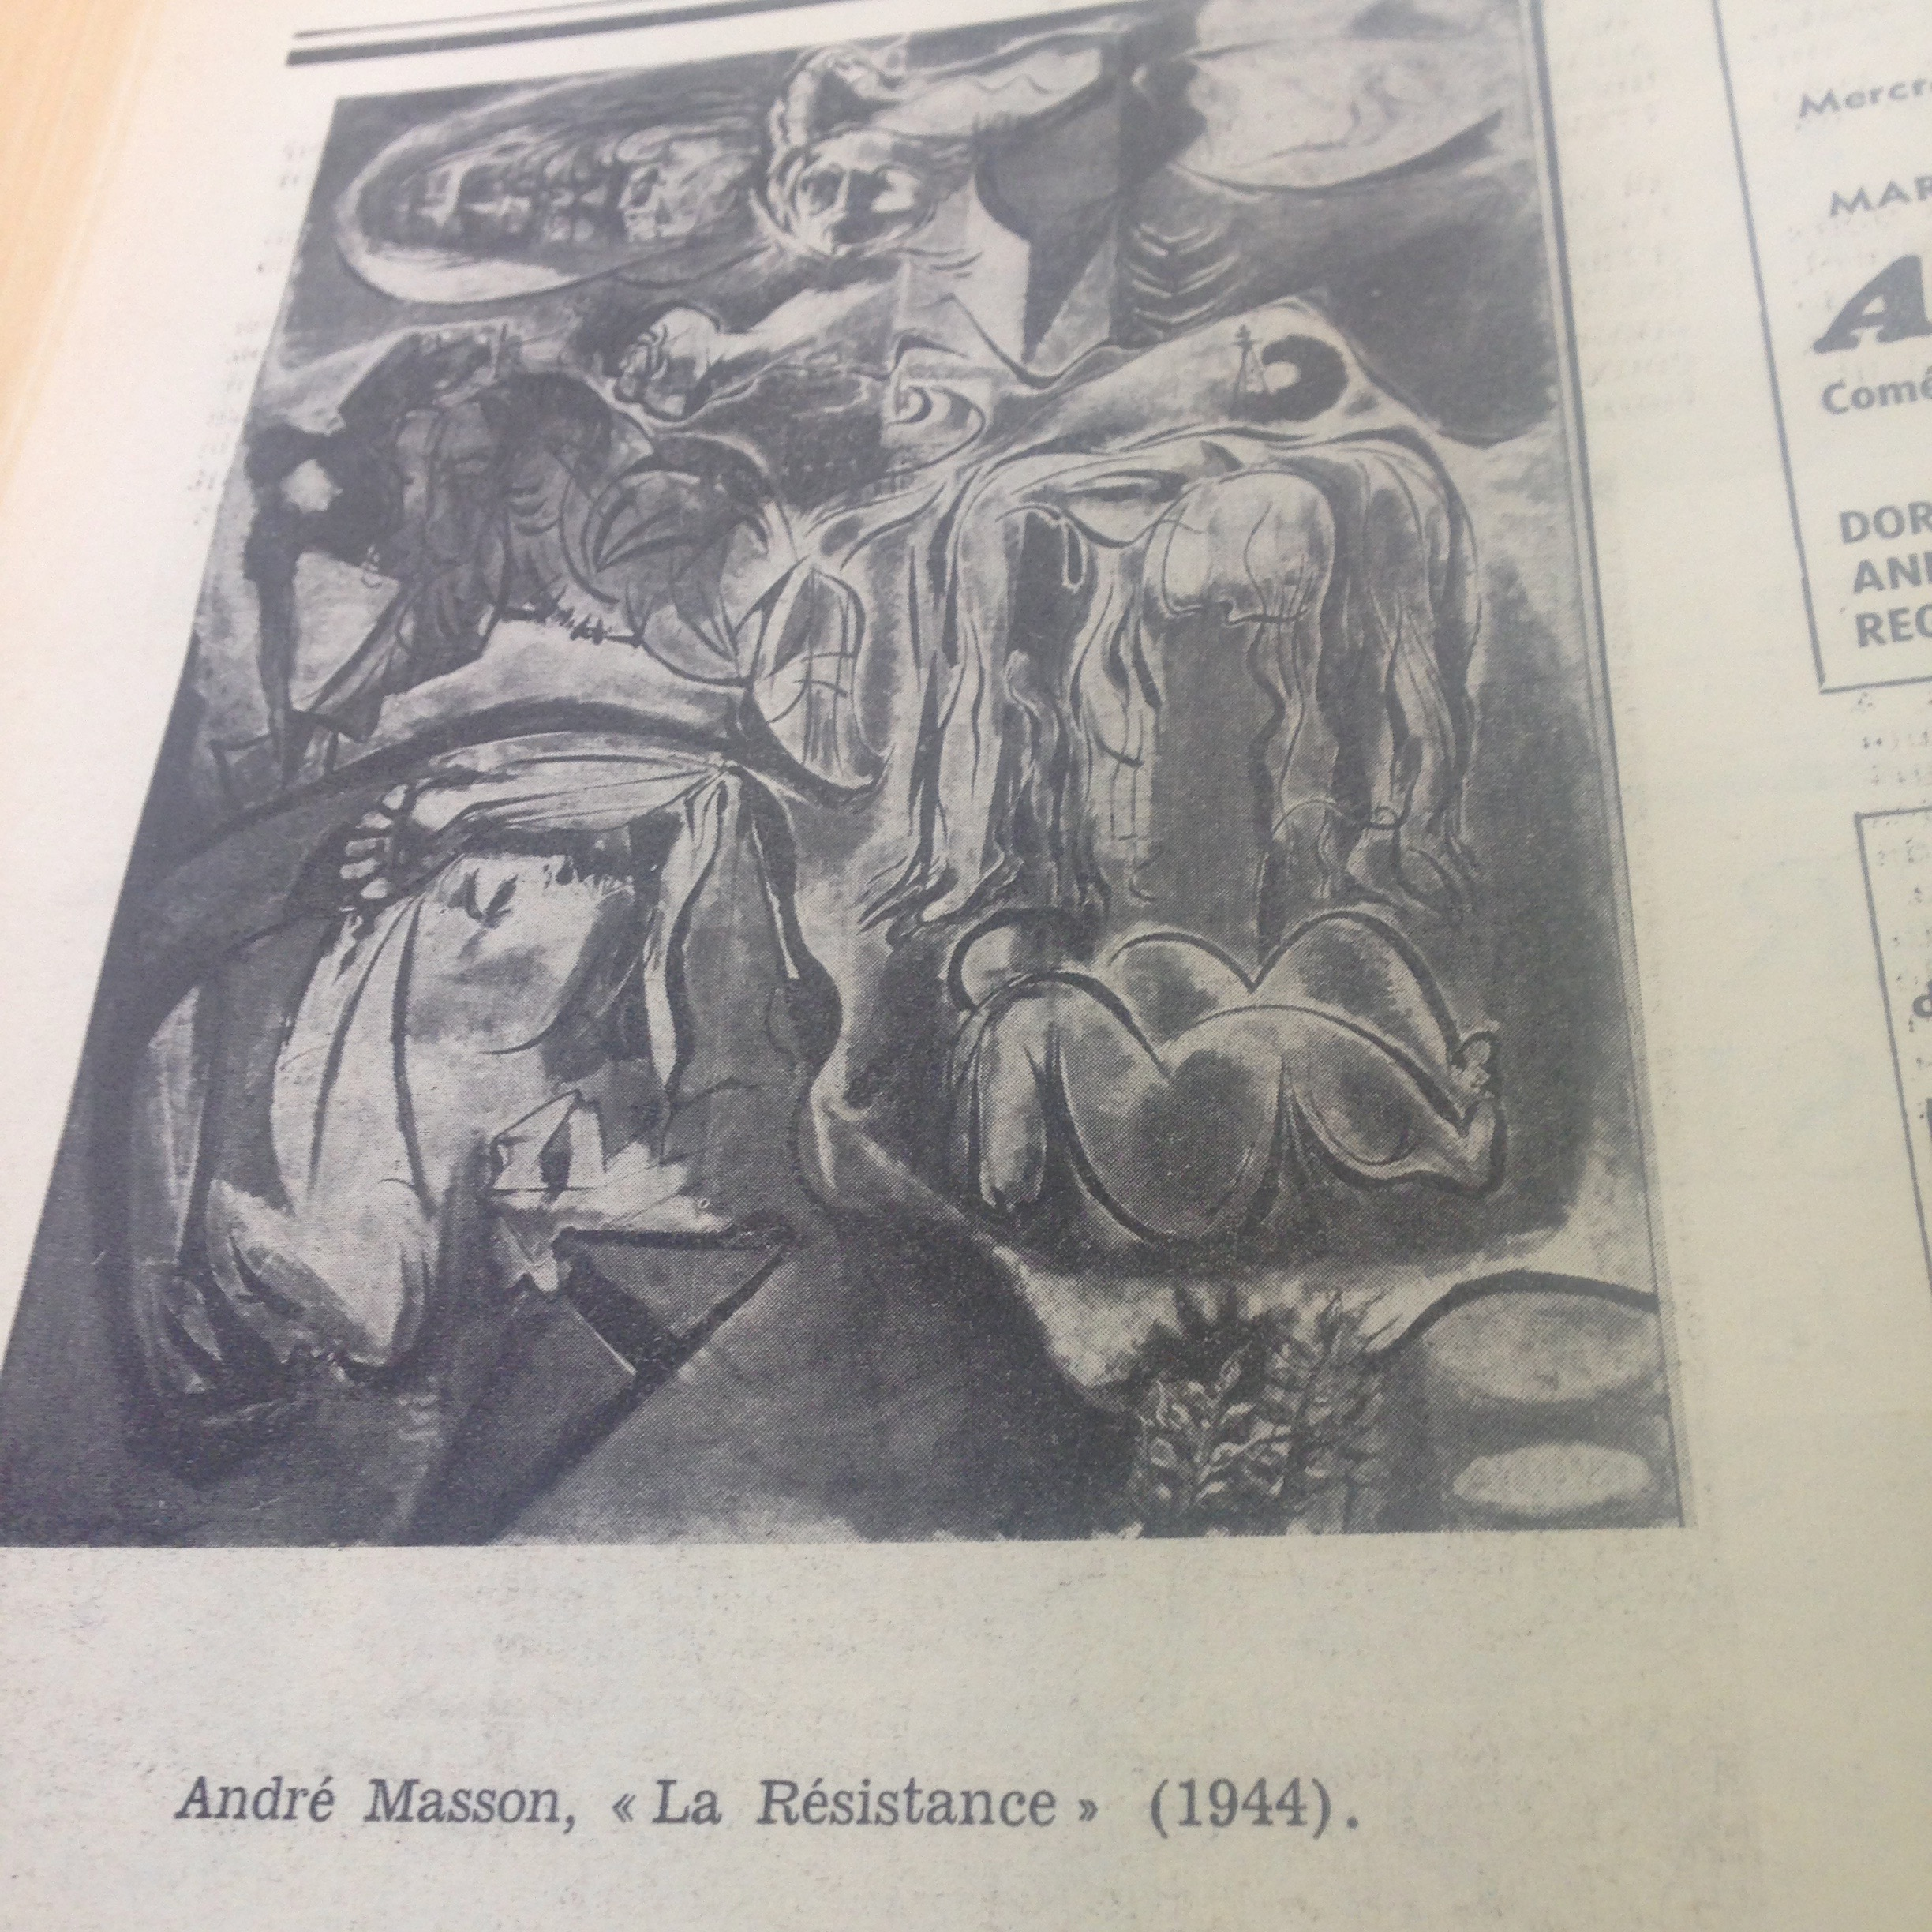
\includegraphics[width=0.33\textwidth]{resistancep2.jpg}
	\caption{\cite{specialelsa}}\label{fig:Réssitance}
\end{figure}

\begin{figure}[H]
   \centering
   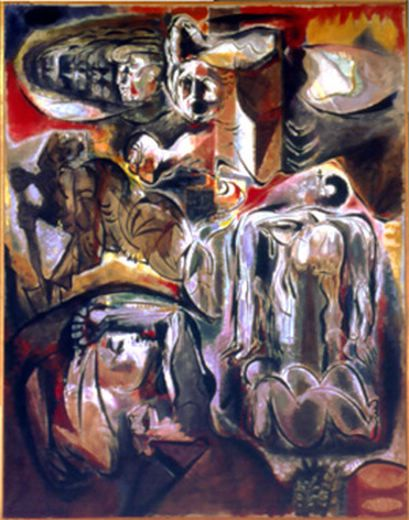
\includegraphics[width=0.33\textwidth]{resistancecouleur.jpg}
	\caption{\cite{specialelsa}}\label{fig:Réssitancecouleur}
\end{figure}



Or, si la Commune est un sujet fidèle et récurrent dans l’ensemble des années des \emph{Lettres françaises}, pas uniquement au moment des anniversaires, et que répertorier les articles sur le sujet conduirait à de riches ressources historiques,l’imaginaire insurrectionnel sous-entendu par cette période historique conduit vers un autre terme qui figure le mot d’ordre du journal. \emph{Les Lettres françaises} naît pendant la Résistance. Il est conçu comme un outil intellectuel au service de cette période spécifique qu’est la Résistance. On peut ainsi concevoir qu’un journal qui doit son existence tout entière à ce moment de l’Histoire et la nature subversive de celui-ci, devenu un passé glorieux après la guerre, fasse du mot « Résistance » la ligne directrice du journal, étant le maitre-mot de sa politique. 


	Ce choix éditorial soulève en lui-même beaucoup de questions, à commencer par l’évolution de la signification du mot \enquote{ésistance}hors l’organisation spécifique de groupes clandestins destinés à s’opposer aux actions de Vichy et des Nazis. C’est la période où André Masson découvre depuis les Etats-Unis \emph{Les Lettres françaises}, dès les premiers numéros, puisqu’il y  fait allusion dans ses correspondances à des articles de 1942. Aussi écrit-il à l’écrvivain Roger Caillois : \enquote{J’ai lu votre très beau texte : “La Pampa“ dans le dernier numéro que j’ai reçu des L.F- Si cette revue ne paraît plus ce sera désolant. (Lettres françaises, n\degre 4, 1er avril 1942, pp. 1-3).}\footcite[p482]{anneessurrealistes} André Masson, comme l’un de ses premiers lecteurs noue donc immédiatement malgré la distance géographique un rapport intime et fidèle aux emph{Lettres françaises}. 


	Aragon, de son côté, participe à sa naissance en opérant la rencontre entre ses premiers dirigeants, Jacques Decour et Jean Paulhan. Par la suite, on s’aperçoit vite que l’évolution du terme \enquote{résistance}, même s’il reste clairement le mot d’ordre, dépend bien sûr des événements historiques à venir, mais aussi de ses dirigeants. Ainsi, lorsque Claude Morgan en prend la direction après la Libération : le mot \enquote{résistance}, de la fin des années 40 et du début des années 50 est  fortement marqué par la Guerre Froide. Symboliquement, ce mot d’ordre est rattaché à la paix. On voit donc dans grand nombre de premières pages de numéros des florilèges de colombes, de Picasso mais pas seulement. Politiquement, résister c’est pour \emph{Les Lettres françaises} de cette période s’opposer à la culture américaine vécue par la ligne éditoriale du journal comme une invasion massive dans le pays. Par opposition, c’est la culture soviétique qui est revendiquée, toujours dans cette finalité qu’est la paix, sous-entendu que le journal en prenant ainsi radicalement parti déclare implicitement que la culture américaine est par opposition celle de la guerre. Ce qui justifie pour glorifier l’URSS la présence d’artistes récurrents tels que le peintre Fougeron ou le dessinateur Taslitzky. Or, l’époque n’explique pas tout, si l’on pense à la reprise du flambeau de la direction des \emph{Lettres Françaises} en 1953 par Aragon et sa politique tant en littérature qu’en art à pluraliser la culture à travers les temps de l’Histoire, mais aussi les différentes parties du monde. Si l’époque pouvait s’y prêter plus facilement, ouvrir le journal à un public qui ne se limiterait pas aux communistes reste un réel choix politique. 


Cependant, il est intéressant de relever que même sous la direction de Claude Morgan en pleine Guerre Froide non seulement la figure d’Aragon exerce une autorité au sein du journal, liée au \enquote{lyrisme populaire} qu’il incarne aux yeux de ses chroniqueurs, mais les révolutions antérieures sont convoquées : celle de 1848 présentée  cent ans plus tard dans un numéro de 1948. L’année même où paraît l’article  \emph{Aragon et l’espérance française} par le philosophe Gilbert Mury. Ainsi, même réfléchie à dessin des intérêts de l’un des camps de la Guerre Froide, la résistance inscrit dans son processus l’étape d’une forme de lyrisme insurrectionnel incarné par les références aux Révolutions. A ce titre, le fameux article du 22 janvier1948 de Gilbert Mury \emph{Aragon et l’espérance française}\footcite{avantgarde} est suffisamment évocateur. La notion d’espoir comprise dans le titre peut d’ailleurs rappeler le numéro du 1er janvier 1948 où le journal appelle ses lecteurs à continuer à croire en l’humanisme. 


Il peut d’ailleurs paraitre symboliquement percutant que sur la première page de ce fameux numéro l’article sur Aragon comme \enquote{espérance}soit accolé à un article à gauche qui parodie les Américains : \emph{Pourquoi serions-nous dupes…puisqu les les Américains n’y croient pas ?}par Yves Farge. Avec une telle mise-en-page, le ton de l’argumentation des articles est donné. Or, dans Aragon et l’espérance française, si Gilbert Mury en associant la figure d’Hugo à Aragon pouvait déjà à la fois évoquer le lyrisme et la période de la Commune de Paris, c’est délibérément avec cette dernière qu’il rassemble Aragon lorsqu’il déclare : \enquote{Le poète Aragon se place délibérément de l’autre côté de la barricade quand il écrit : “Ils sont la force et nous sommes le nombre“ ou bien : “Ma patrie est la faim, la misère et l’amour“.}

%Source pour image : Les Lettres françaises [n°192-27 janvier 1948] "Pourquoi serions-nous dupes...Puisque les Américains n'y croient pas ?" par Yves Farge.

\begin{figure}[H]
   \centering
   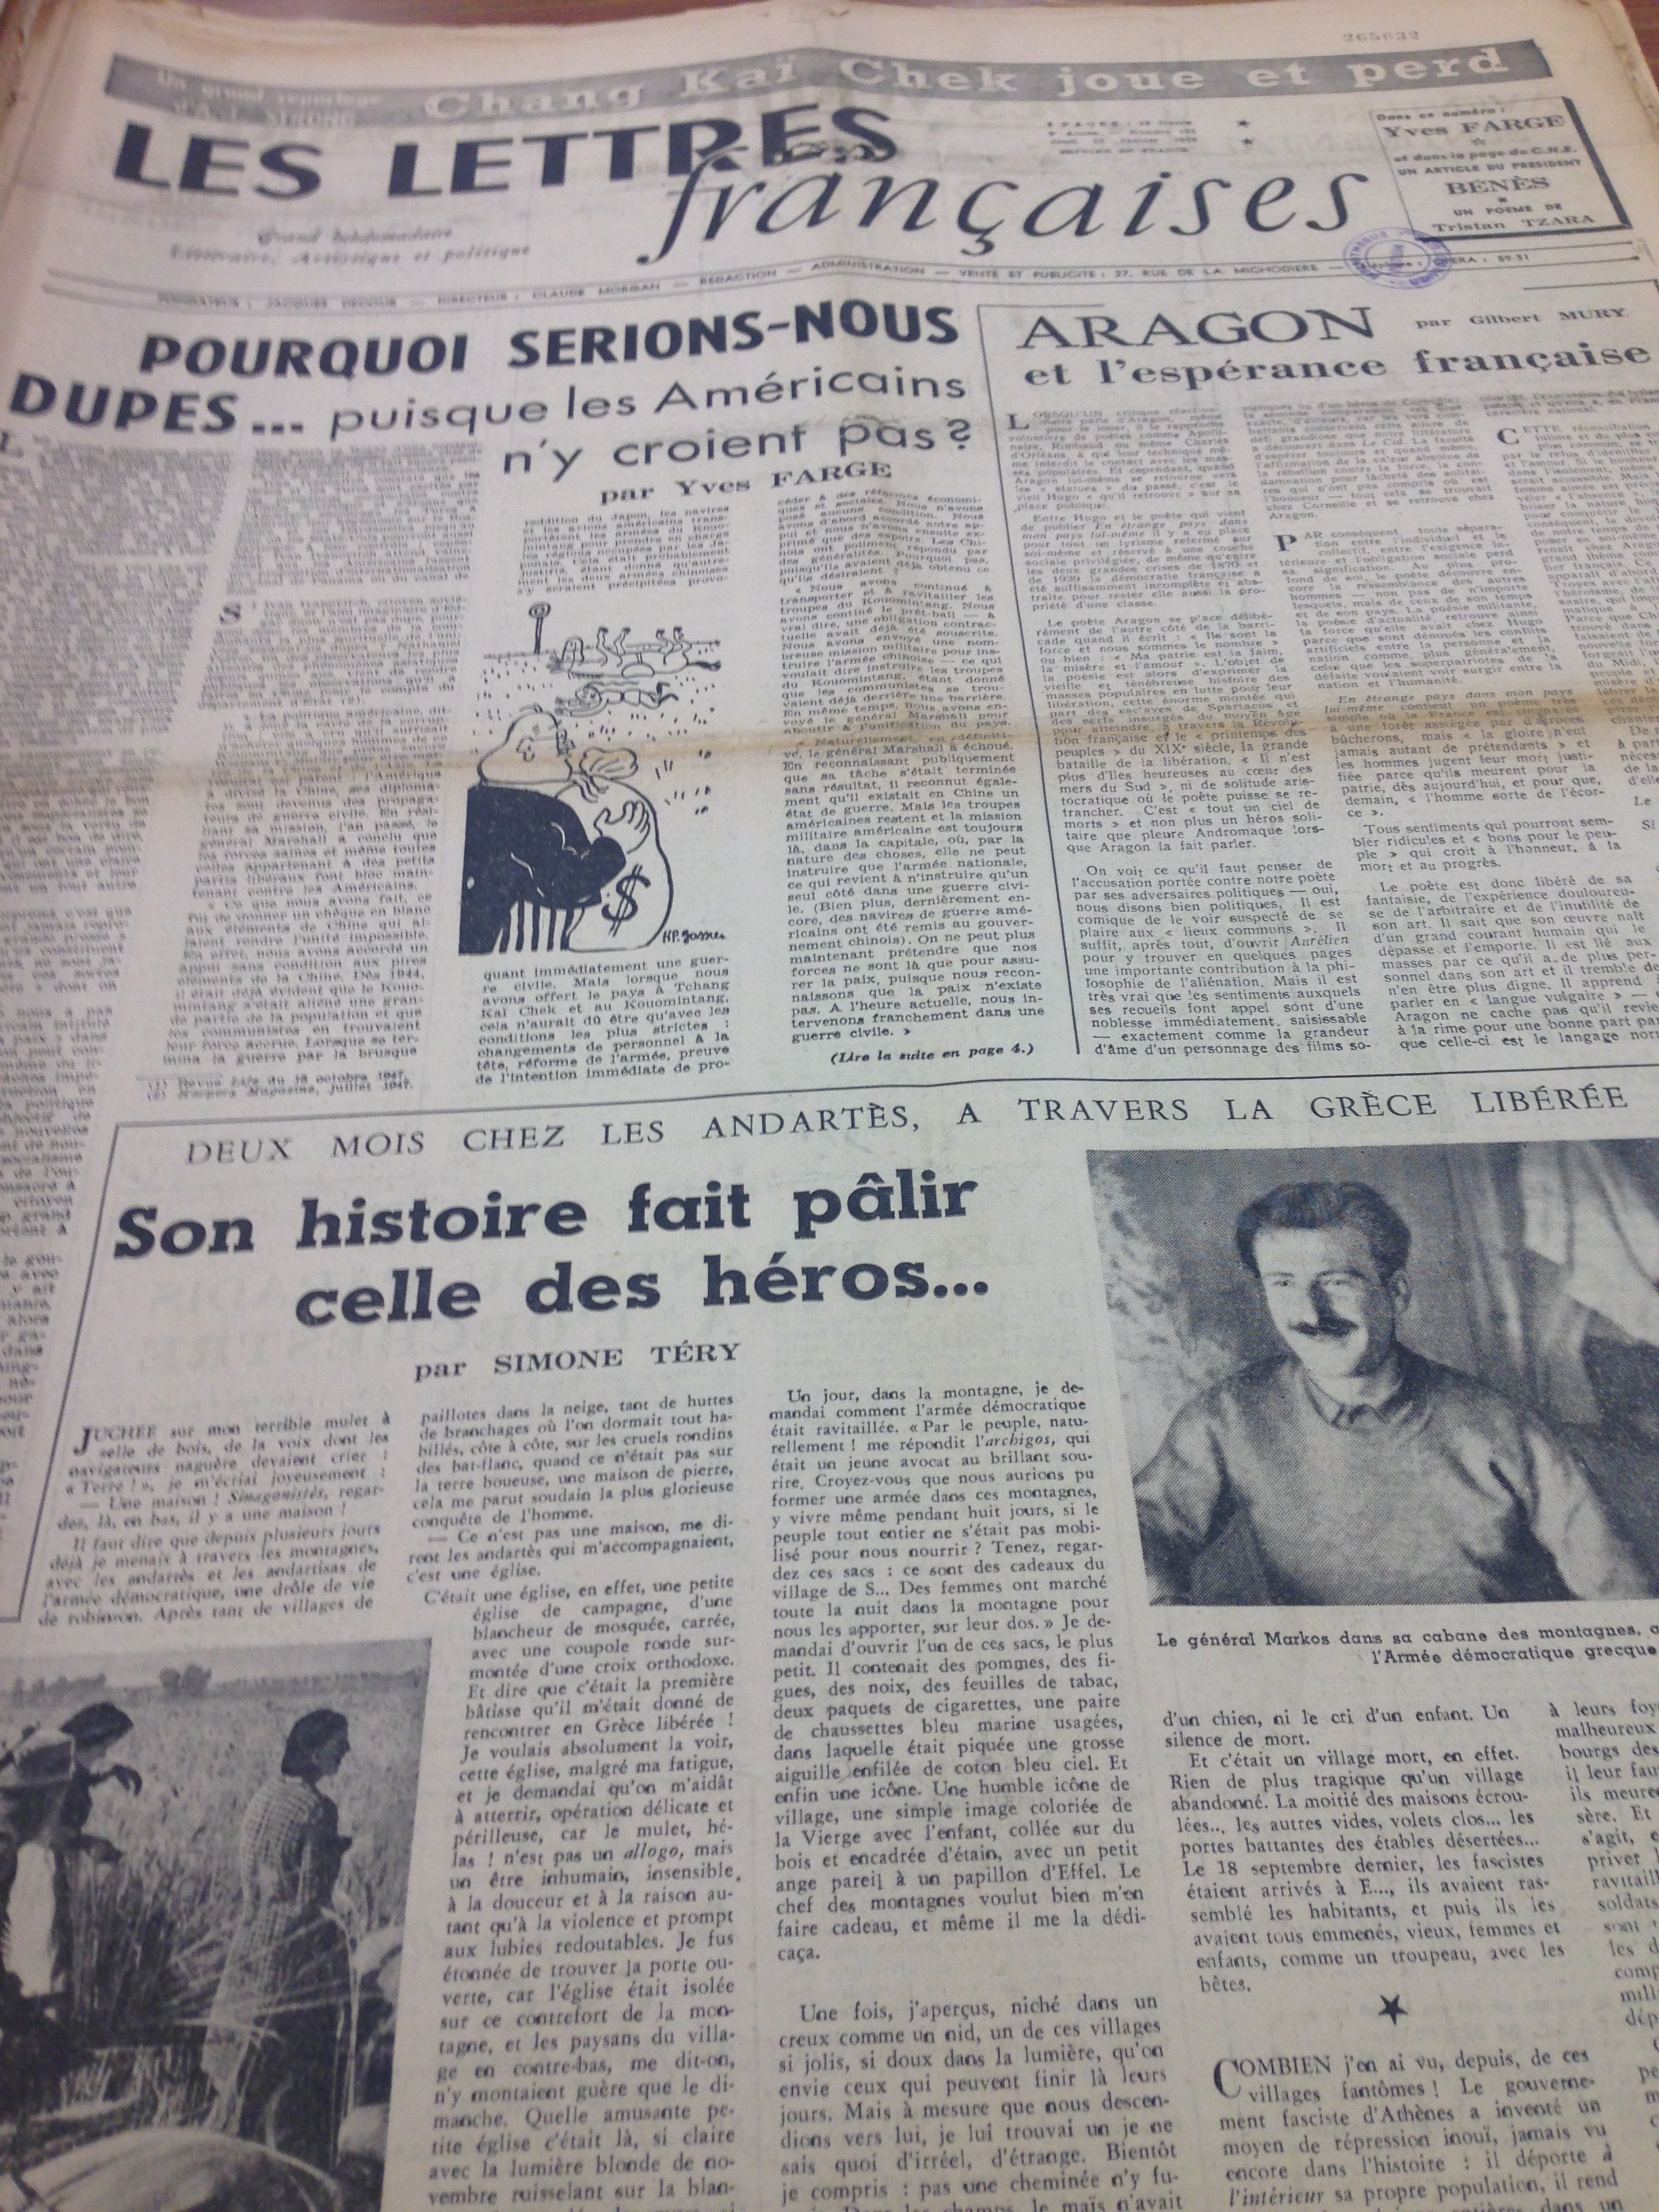
\includegraphics[width=0.33\textwidth]{27janvier1948.jpg}
	\caption{\cite{journallimbour}}\label{fig:}
\end{figure}


	D’une part, Mury emploie la métaphore des barricades, qui dans l’imaginaire collectif rappelle l’épisode de la Commune de Paris. D’autre part, il prête à la Commune un aspect romantique lorsqu’il extrait des fragments des poèmes \emph{Richard Coeur de Lion} et \emph{Plus belle que les larmes}, deux poèmes du recueil \emph{Les yeux d’Elsa}. La figure de la femme aimée se trouve ainsi mêlée à  celle de la patrie. Que le propos politique de l’article ait une portée romantique se confirme d’autant plus avec la seule allusion à une oeuvre romanesque d’Aragon, \emph{Aurélien}. Si Aragon est d’ailleurs désigné dans l’article avant tout comme poète, c’est aussi pour pointer une forme qui reflète le romantisme insurrectionnel : \enquote{Aragon ne cache pas qu’il revient à la rime pour une bonne part parce que celle-ci est le langage normal courant, l’expression du lyrisme populaire et qu’elle a, en France, un caractère national.}

	Toutefois, on ne peut ignorer le double enjeu du message de Mury, qui ne vise pas seulement à louer le lyrisme révolutionnaire, mais aussi à opposer celui-ci contre les Américains, c’est-à-dire par opposition au gros banquier américain caricaturé à côté de son article, lui bien loin de toute forme insurrectionnelle ou poétique avec son gros sac de dollars dans les mains. C’est pourquoi Mury en appelle en partie contre les Américains par la biais du lyrisme patriote. Que les choix de fragments de vers d’Aragon proviennent du recueil d’Aragon écrit pendant la Résistance s’inscrit directement dans la politique éditoriale du journal. 

Cependant, Mury attribue à l’imaginaire romantique d’Aragon son origine au coeur de la lutte des peuples et son apothéose qu’a été la Révolution Française : 

\begin{quote}
 L’objet de la poésie est alors d’exprimer la vieille et ténébreuse histoire des masses populaires en lutte pour leur libération, cette énorme montée qui part des esclaves de Spartacus et des serfs insurgés du moyen âge pour atteindre à travers la Révolution française et le “printemps des peuples“ du XIXème siècle la grande bataille de la libération.   
\end{quote} 

 La synthèse de l’histoire de ces révoltes suit clairement la ligne de peuples en révolte, c’est-à-dire en situation de résistance face à l’oppresseur. On pourrait d’ailleurs substituer à l’\enquote{espérance française} le terme \enquote{résistance} lorsque Mury conclue : 

 L’espérance française apparait ainsi avec ses objectifs bien précis de lutte contre l’envahisseur, et plus largement de défense matérielle et morale du pays. Elle est, comme la poésie d’Aragon elle-même, la forme que revêt la France depuis 1939 et pour longtemps encore l’affirmation exigeante, agressive, quotidienne d’un infini purement humain et inséparable de l’homme.

	 En somme, l’\enquote{espérance française}, c’est la Résistance. Et Aragon, en est à la figure d’autorité par excellence, d’autant plus avec le réalisme socialiste, sa fonction purement patriotique, qu’il incarne par opposition à l’invasion culturelle américaine ressentie par les dirigeants des \emph{Lettres françaises}. 
\subsection{La place d'André Masson dans la politique de la Guerre Froide}

     Quel rôle joue la figure d’André Masson dans \emph{Les Lettres françaises} au moment où la Résistance veut jouer un rôle partisan de la patrie pendant la Guerre Froide ? Un entretien d’André Masson relaté par Claudie Planet\footcite{entretienmasson} est publié en mars 1949. Bien qu’André Masson ne puisse pas directement s’inscrire dans le combat mené par la direction du journal contre la culture américaine, il est intéressant de relever qu’André Masson déclare lui-même être en pleine période d’évolution de perspective de son art. L’article est d’ailleurs accompagné de deux photographies : La première perceptible est l’illustration d’une peinture d’André Masson de 1947, \emph{Portrait de l’artiste par lui-même}. La seconde est une photographie de Masson de dos en train de peindre sur la toile. Il est donc intéressant de relever qu’au moment où le journal \emph{Les Lettres françaises} démarre sa campagne à la gloire de la culture soviétique contre les Américains, André Masson s’établit, après son exil aux Etats-Unis pendant la guerre, en Provence. On imagine quel changement de regard s’opère pour cet exilé de retour en France. Peut-être cet entretien est-il d’ailleurs, sinon la première, l’une des premières collaborations d’André Masson avec le journal.
	 
\begin{figure}[H]
   \centering
   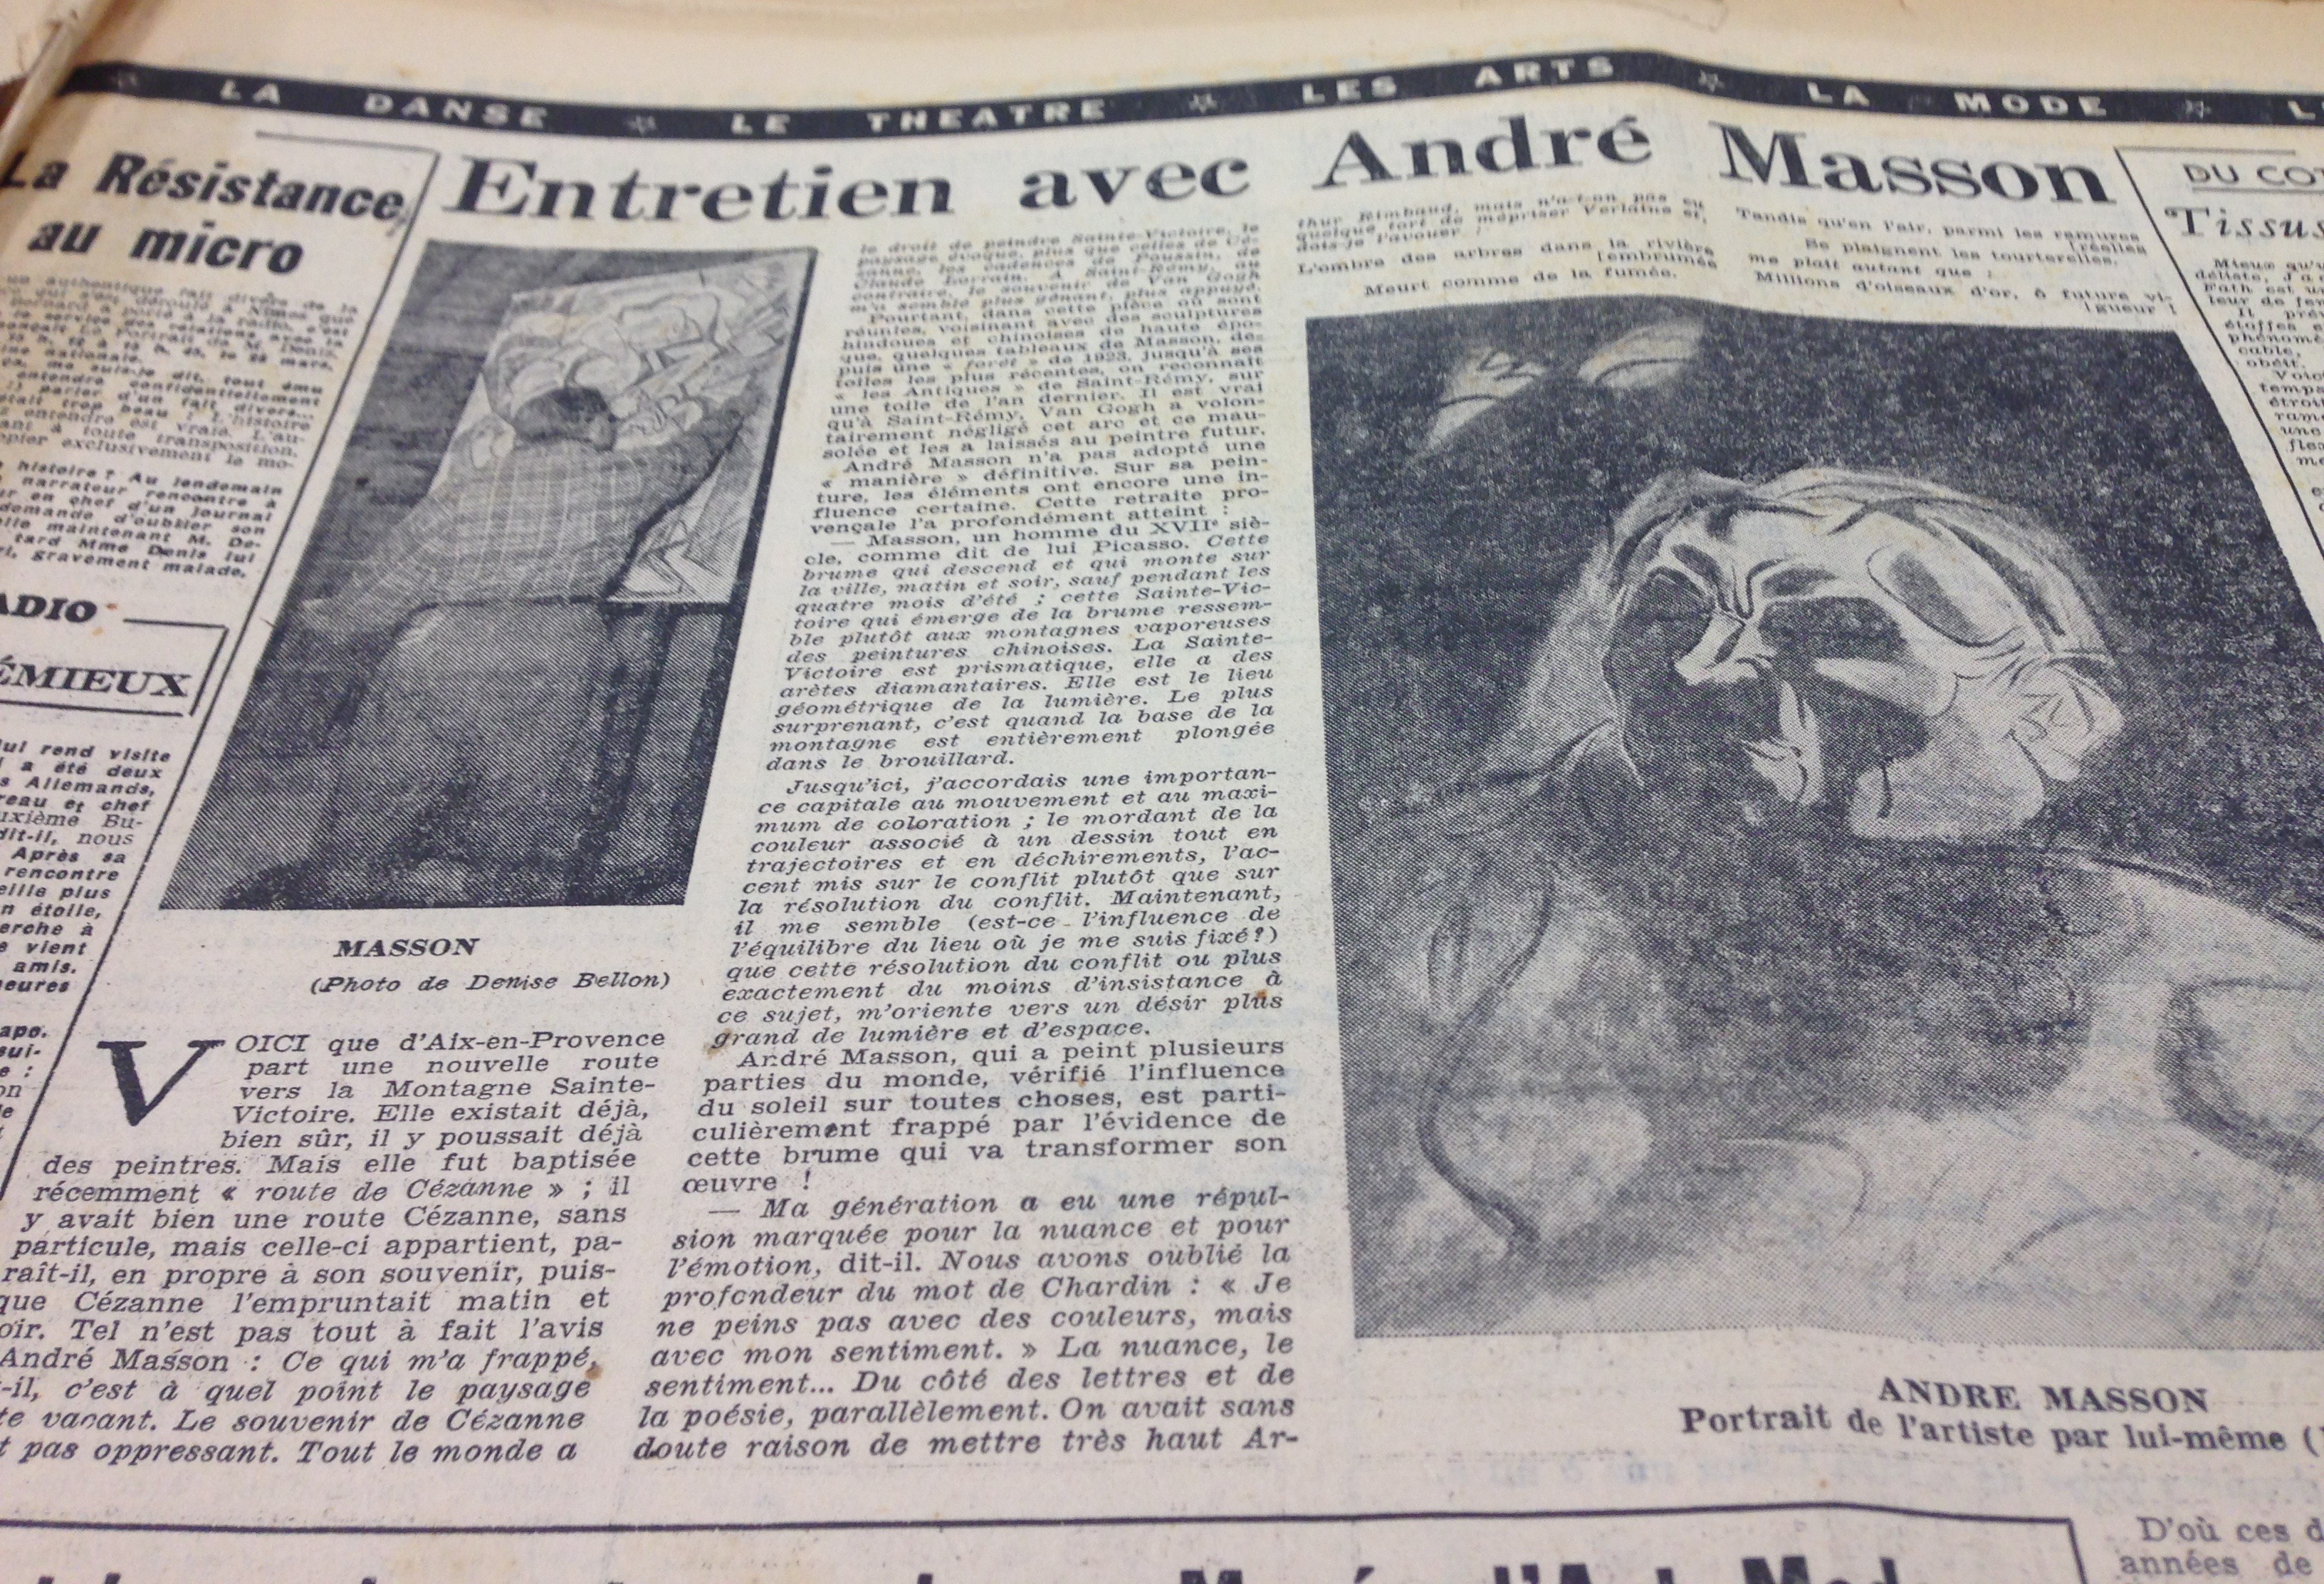
\includegraphics[width=0.33\textwidth]{pageplanet.jpg}
	\caption{\cite{entretienmasson}}\label{fig:Planet}
\end{figure}


Or, force est d’admettre que de ce déplacement de regard le message politique ne peut plus être tout à fait le même : 
\begin{quote}
  Jusqu’ici, j’accordais une importance capitale au mouvement et au maximum de coloration; le mordant de la couleur associé à un dessin tout en trajectoires et en déchirements, l’accent mis sur le conflit plutôt que sur la résolution du conflit. Maintenant, il me semble (est-ce l’influence de l’équilibre du lieu où je me suis fixé ?) que cette résolution du conflit ou plus exactement du moins l’insistance à ce sujet, m’oriente vers un désir plus grand de lumière et d’espace.  
\end{quote}
 

	Non seulement c’est André Masson lui-même qui marque avec ses propres mots une nouvelle étape dans son art, mais il semble distinguer en substance celle-ci, lorsqu’il évoque les \enquote{conflits} de sa série de dessins \emph{Massacres} des années 1930. En réalité, ce n’est pas tant le message politique qui change que le déplacement de perspective. C’est pourquoi, même si André Masson est clairement à rebours du conflit politique qui occupe l’esprit des \emph{Lettres françaises} de cette fin des années 40, lui aussi se plonge dans une période de transition. On peut d’ailleurs relever un brin d’ironie entre le choix de l’autoportrait de Masson choisi pour le présenter par le journal vis-à-vis des nouvelles considérations esthétiques évoquées dans l’entretien : Si Masson concède dans l’entretien posséder « deux faces », la lumière et l’obscurité, et sa préférence en train d’advenir pour la lumière, Claude Planet conclue en précisant \enquote{tout ce que vient de nous dire Masson est confirmé soudain par cette vapeur qui trouble leur netteté et qu’il est impossible de ne pas voir.} Comme si l’attrait de Masson de la lumière résiderait dans cette exploitation du \emph{sfumato}. 


\begin{figure}[H]
   \centering
   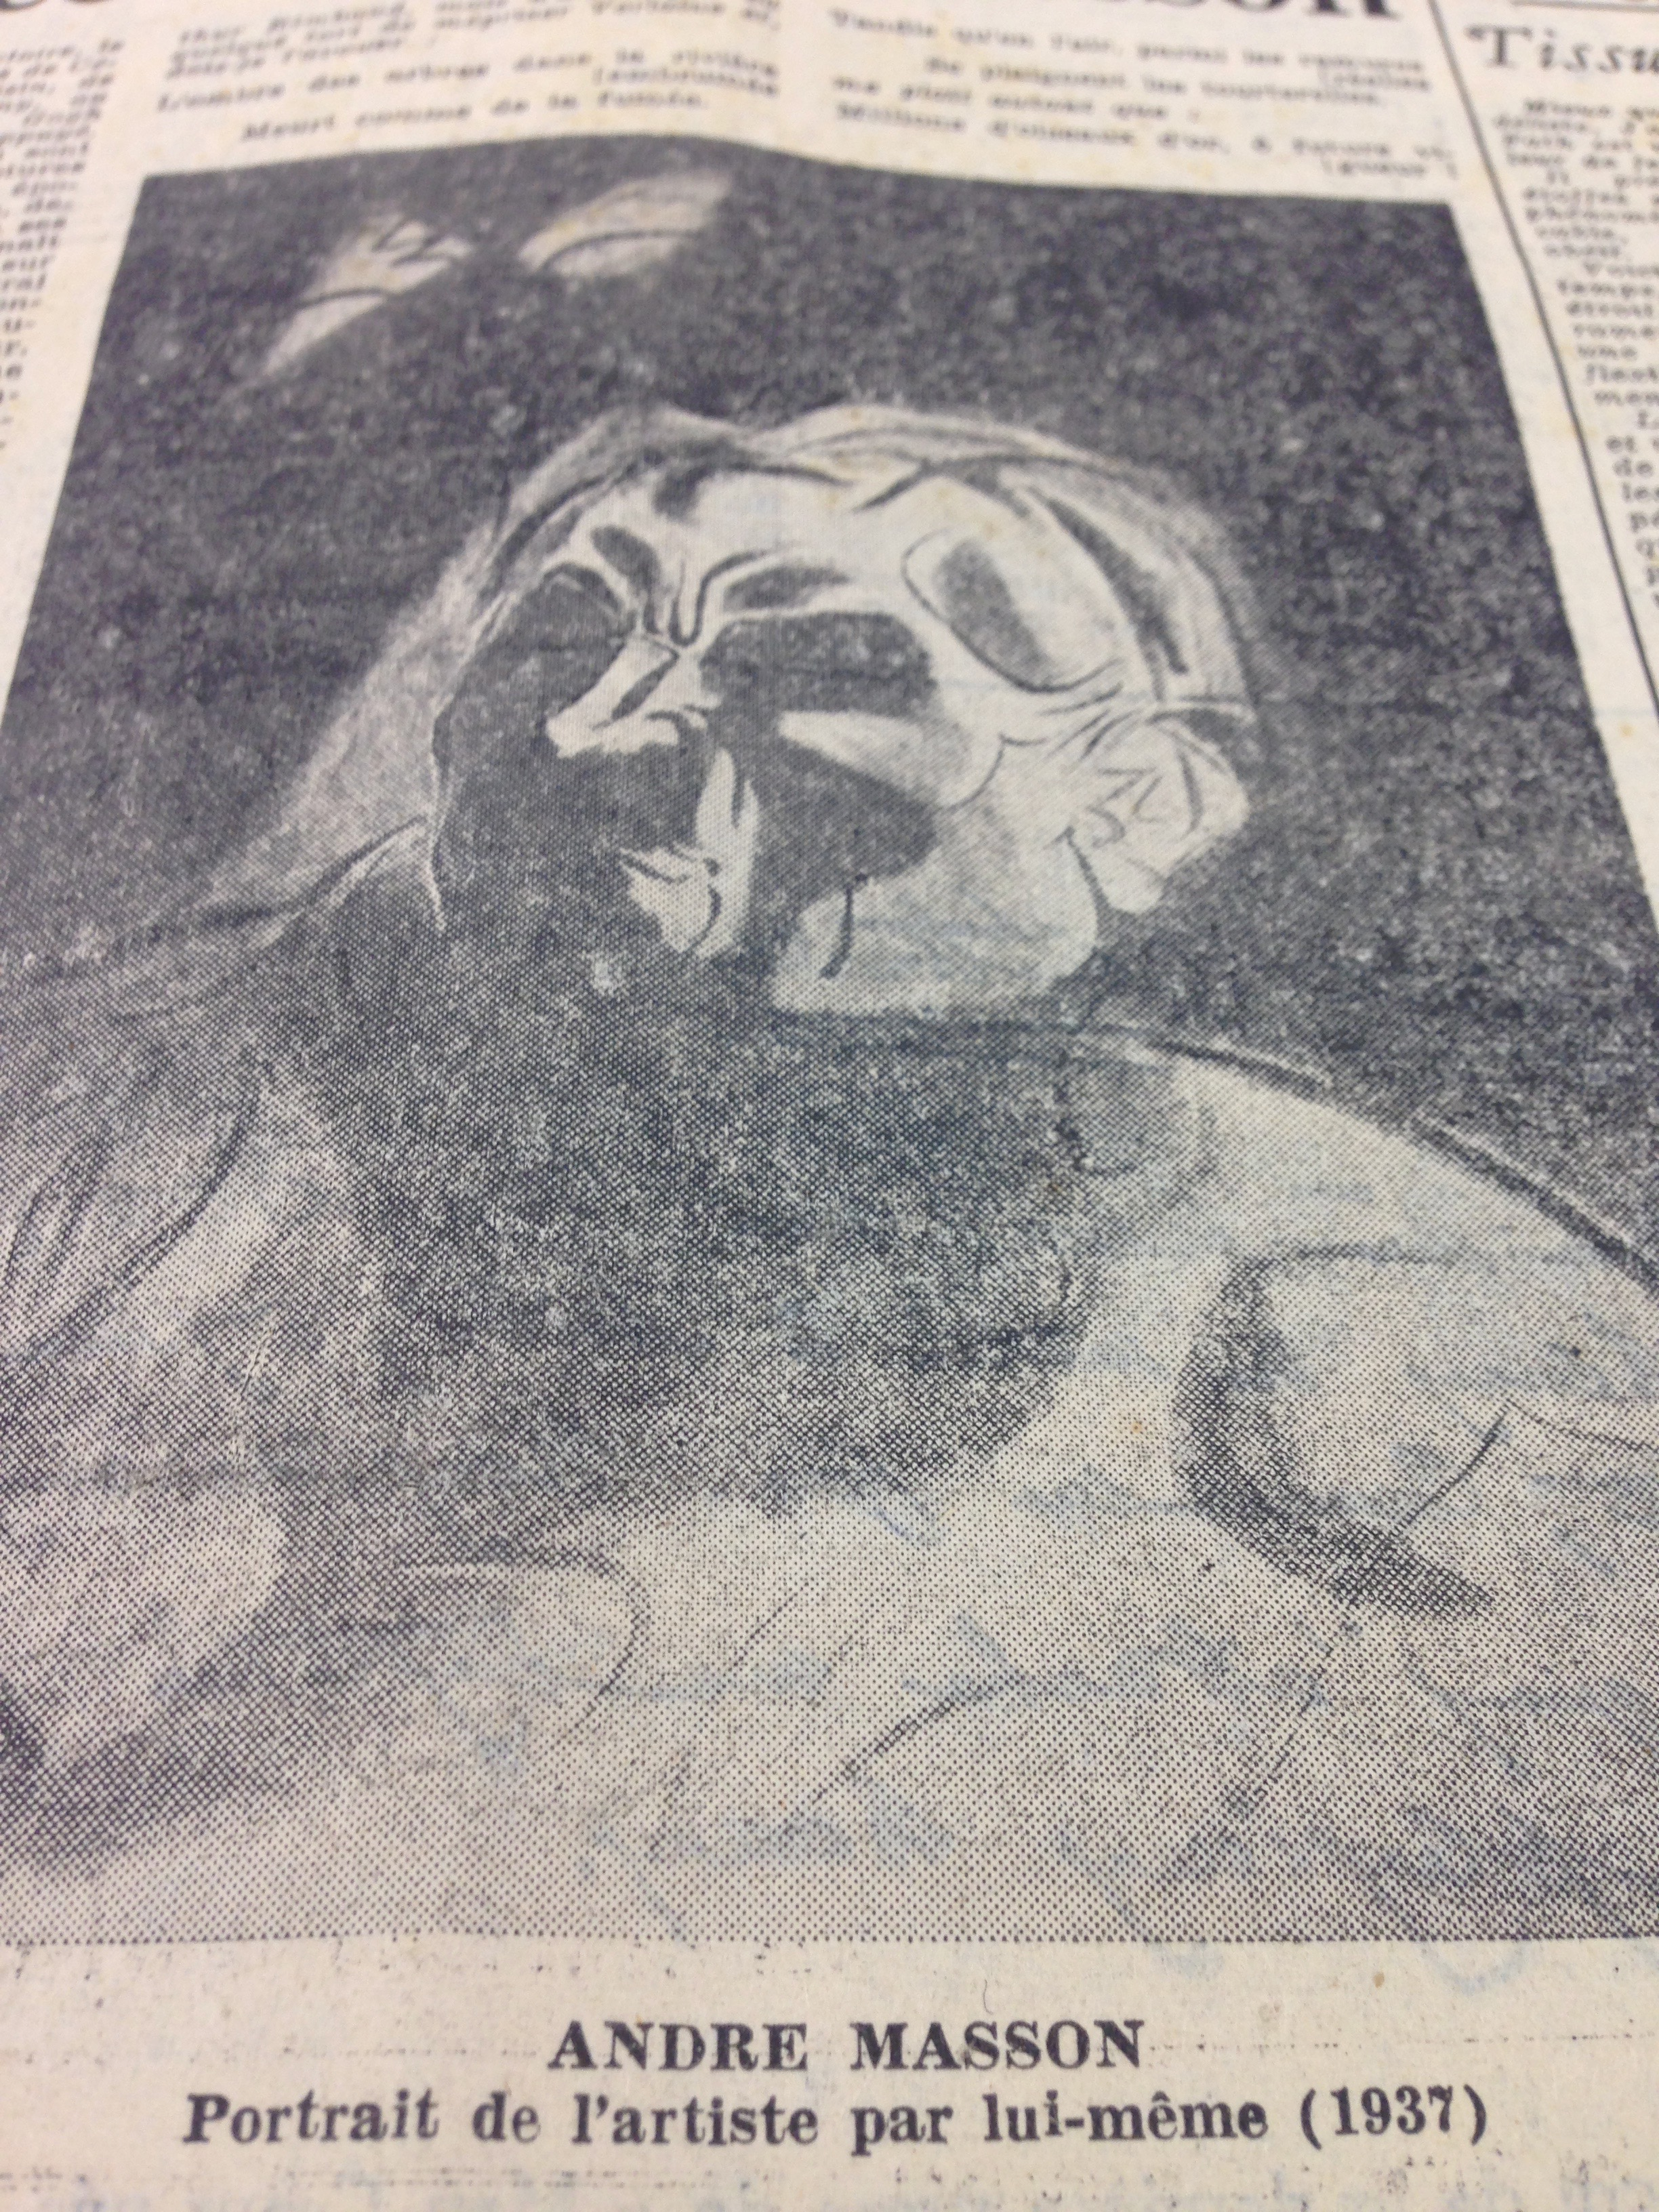
\includegraphics[width=0.33\textwidth]{artistemasson.jpg}
	\caption{\cite{entretienmasson}}\label{fig:Autoportrait}
\end{figure}

\begin{figure}[H]
   \centering
   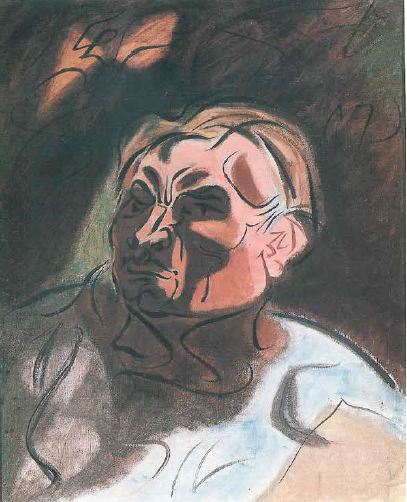
\includegraphics[width=0.33\textwidth]{massoncouleur.png}
	\caption{\cite{entretienmasson}}\label{fig:Autoportraitcouleur}
\end{figure}


Néanmoins, bien que l’autoportrait de Masson soit reproduit en noir, et blanc, les couleurs originelles peuvent interpeller après ce discours de Masson : A l’inverse de l’entretien, le décor est du côté de l’obscur avec un jeu d’ombre à l’arrière-plan avec des teintes de rouge vif similaires à la couleur du visage, plus proche d’un masque que d’un visage humain. Or, c’est la lumière qui transperce ce décor sombre. L’autoportrait de 1947 agit donc exactement à l’inverse des attirances esthétiques que provoque la Provence chez Masson. Mais, si l’obscurité fait surgir la lumière, et la lumière provençale la brume, quel est le véritable élément des deux l’origine du désir du Masson de cette période ? Toujours est-il que, si André Masson ne peut pas participer comme le ferait Fougeron directement dans la bataille des \emph{Lettres françaises }contre la culture américaine, même si lui n’appelle pas directement à la paix, son témoignage sous-entend qu’il recherche ainsi lui cette fois la \enquote{résolution} du conflit. Sans que Masson se confonde dans le parti pris du journal, une proximité intellectuelle se tisse.  

\section{Les enjeux de la politique éditoriale : [n\degre1085- du 17 au 23 juin 1965] et  [n\degre1100- du 7 au 14 octobre 1965] :}

subsection{Les correspondances entre le journal et l'oeuvre romanesque}

Comment la résistance évolue-t-elle au moment des grandes innovations éditoriales ? Quel rôle joue la résistance nourrie par la réflexion des mediums qu’à la direction des \emph{Lettres françaises} en 1965 sur son propre journal ? Deux ans avant \emph{Blanche ou l’oubli}, la direction en annonçant en première page les raisons du prochain format et organisation des numéros à venir à la rentrée de l’automne, l’aspect médiatique est au coeur de la question du changement adapté aux considérations idéologiques du journal :

\begin{quote}
Aussi important est l’essor de la télévision et ses perspectives immédiates, par exemple. Mais l’expansion des sciences, de toutes les sciences humaines, comme de la nature, le progrès prodigieux des techniques, font que la véritable source de multiplication se trouve dans les transformations inégalées tant en ampleur qu’en rapidité de notre vie, de nos conceptions, de notre psychologie. Un journal comme le nôtre n’a de sens que s’il est capable de refléter ces changements.\footcite{nouvelleformule}\end{quote}


	Tout un pan de la politique éditoriale cherche à s’ancrer dans les évolutions de la société, en particulier technologiques, mais aussi pour les conséquences réceptives, émotives, qui en résultent.

\begin{figure}[H]
   \centering
   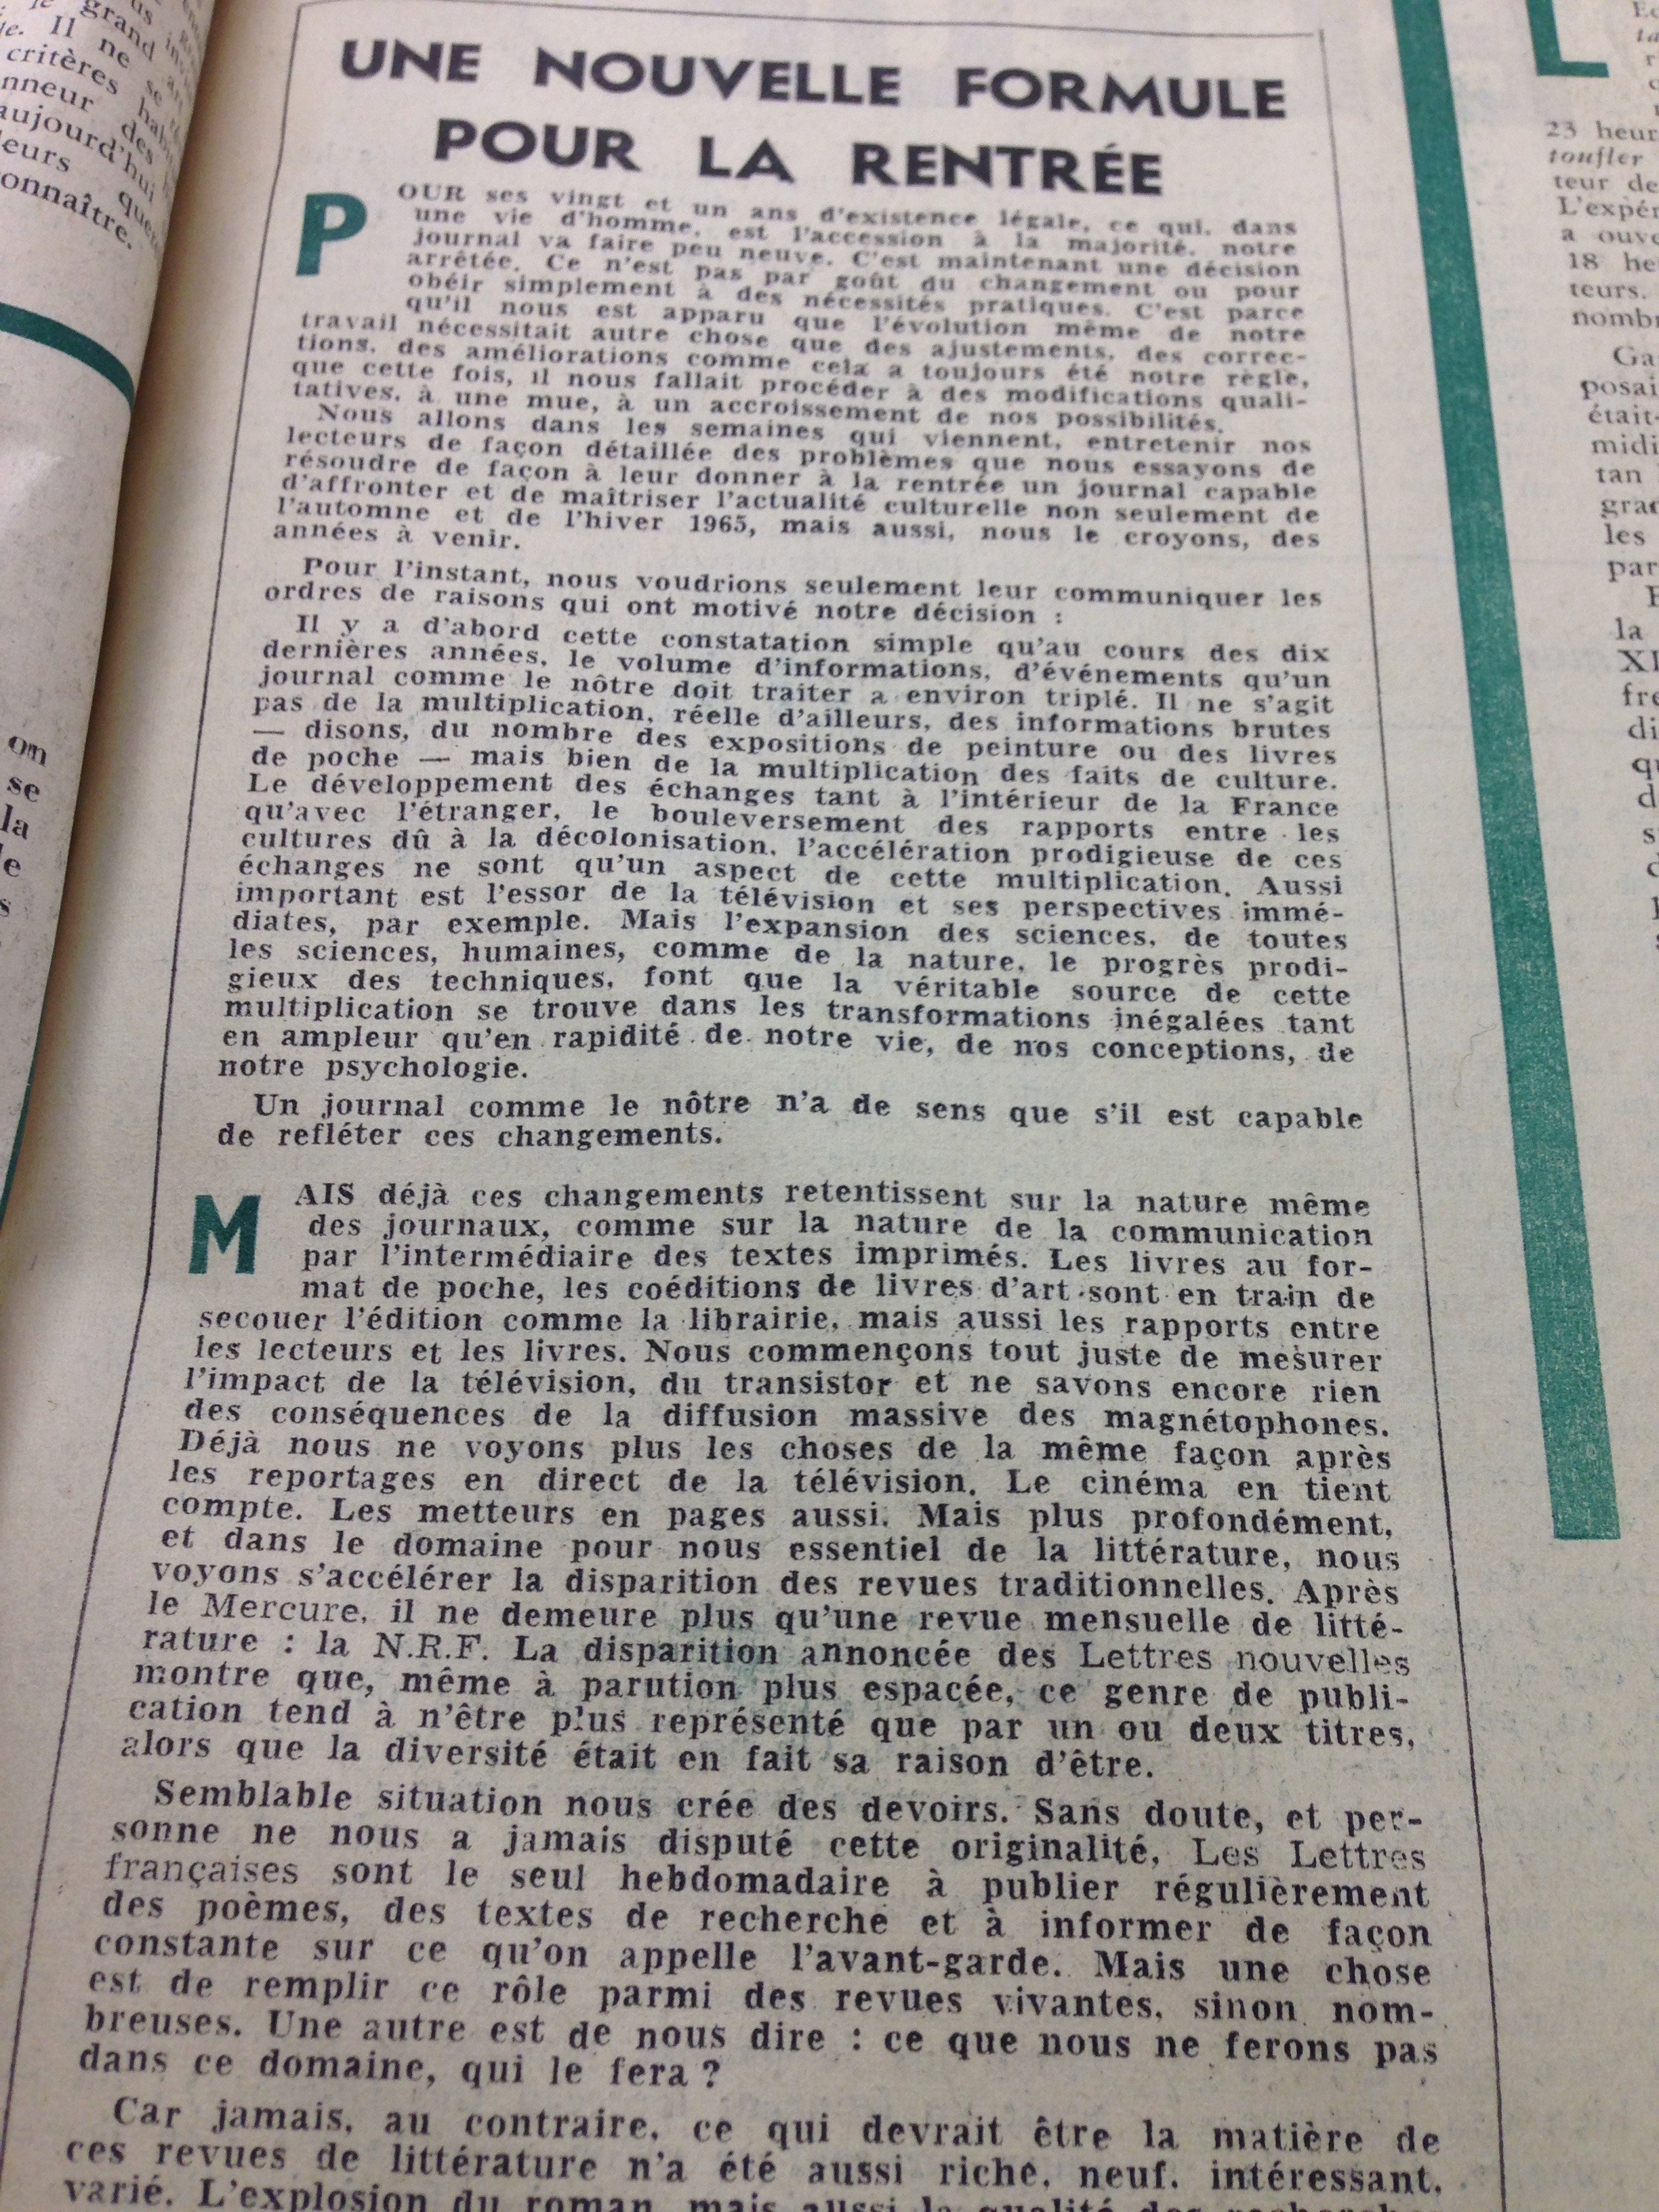
\includegraphics[width=0.33\textwidth]{nouvelleformuleannonce.jpg}
	\caption{\cite{nouvelleformule}}\label{fig:annoncenvformule}
\end{figure}


	C’est pourquoi en même temps que l’aspect de la politique éditoriale des \emph{Lettres françaises}, on pourrait facilement croiser la réflexion pour la prochaine formule des numéros à venir et celles romanesque de \emph{Blanche ou l’oubli}. Ouvrage de 1967 mais dont l’action a lieu en 1965. Le point commun essentiel réside dans le constat d’Aragon des évolutions technologiques et de la révolution dans ce domaine que cette période est en train de vivre, et paradoxalement ce que produit cette intelligence collective comme lien intime sur l’homme en tant qu’individu. La résistance au sens d’Aragon comme directeur des \emph{tLettres françaises} en 1965, c’est encore une fois un processus qui prend en compte l’étape de transformation qu’est la révolution, mais sous diverses formes, y compris celle de transformer le journal en fonction des changements de perceptions sur les individus que sont en train de produire les développements technologiques sur les individus.

	 En outre, la Résistance est directement déplacée dans \emph{Blanche ou l’oubli} dans la perspective des nouvelles technologies et de la réception qu’elles provoquent : \enquote{“- Oh ! - il fait, Philippe -, tu la ramènes, avec la Résistance. Cette année, c’est bien simple, la télé n’était pas visible !“}. La tonalité humoristique n’exclue en rien la prise en compte par Aragon de cette génération venue après lui qui n’a pas vécu cette période historique. C’est donc aussi la jeunesse qui est interpellée dans la réflexion d’une nouvelle formule du journal, celle à qui Aragon entend parler en tant qu’auteur et directeur de journal. 

	Cette idée rejoint l’autre grand mot d’ordre propre plus à Aragon probablement qu’à son prédécesseur Claude Morgan, qui serait de joindre le passé de résistance à la pluralité. A ce titre, Aragon voit en son lecteur également un spectateur, d’où la prolifération d’images et pas seulement dans les rubriques d’Art, mais aussi comme individu dans l’ère de son temps. Si cette réflexion sur l’évolution technologique rencontre la fameuse question des Livres de poche, cette pensée de la direction rappelle une fois encore la pensée du prochain roman d’Aragon, riche des grandes enquêtes de 1964 entreprises par \emph{Les Lettres françaises} sur le livre de poche : \enquote{Marie Noire oublie la comète, oublie sur un guéridon son \emph{Livre de poche}, elle se lève et se voit, s’imagine dans le miroir au-dessus de la cheminée} , ou encore :
	\begin{quote}
	 Marie Noire n’a pas lu la Correspondance, on n’en est pas encore à en faire des romans d’espionnage, je veux dire des Livres de poche. Elle se regarde dans la glace, et elle y voit au fond, tout nu, assis sur ses jambes, ce garçon qui lui a dit je t’aime.\footcite[p102]{blancheouloubli}\end{quote}

	  On ne peut ignorer que ces deux références à la même page au livre de poche précèdent directement une autre référence-clé chez Aragon, particulièrement visible en cette année de 1965 avec \emph{La mise à mort}, le miroir. L’intelligence des machines d’une part, celle du livre de poche d’autre part, comme reflet de l’homme. 


Mais l’échange entre ces numéros et le roman à venir ne s’arrête pas-là. Cette réflexion au coeur de \emph{Blanche ou l’oubli} existe non seulement comme enjeu de politique éditoriale dans la nouvelle formule de 1965, mais les numéros qui font allusion à cette fameuse nouvelle formule du journal \emph{Les Lettres françaises} existe eux-aussi comme allusions dans \emph{Blanche ou l’oubli} : \enquote{Ce n’est pas très important, et il est vrai que ce roman n’a été inclus dans le Livre de poche qu’au mois de juin 1965. Pas cinq mois. ça suffit pour qu’en octobre…}. En faisant allusion à la parution de \emph{L’Education sentimentale} en livre de poche, le narrateur mentionne le mois de « juin 1965 », qui est celui où \emph{Les Lettres françaises} annonce en première page réfléchir à une nouvelle formule du journal à compter de la rentrée d’octobre. Et c’est justement dans le numéro du 7 octobre 65 que parait la fameuse nouvelle formule. Peut-on voir ainsi dans cette rêverie autour du Livre de Poche un clin d’oeil à ces deux numéros précisément qui en plus le livre de poche comme modèle d’une nouvelle formule du journal publient dans le numéro suivant la suite de l’article \emph{Une nouvelle formule pour la rentrée (II), La révolution du livre }? Quoi qu’il en soit, la politique éditoriale du journal, à partir de son mot d’ordre de résistance, dérive par de multiples axes jusqu’à réapparaître et retrouver leurs réflexions poursuivies dans les oeuvres romanesques même d’Aragon. Un jeu de correspondance s’établit donc entre le journal et les romans, ainsi qu’un autre niveau de lecture où le roman fait allusion aux articles des \emph{Lettres françaises}. 


\subsection{Masson comme médiateur entre Elsa et la Résistance}

En comparaison, le rapport d’André Masson à la Résistance n’est pas similaire à celui d’Aragon. Ce dernier, en tant que poète et  directeur du journal, dans un numéro de  1965,  revenait encore  sur la naissance du journal \emph{Les Lettres françaises} et du CNE\footcite{histoirecnetriolet}, l’autre grande création pendant la Résistance\footcite{specialelsa} dans laquelle Aragon et Elsa Triolet jouent un rôle de premier plan. Néanmoins, un numéro de 1971 très particulier exploite le ressenti d’André Masson face à la Résistance : Il s’agit d’un numéro spécial en hommage à la mémoire Elsa. Mais, au-dessus-de la banderole verte des \emph{Lettres françaises}, un autre sujet cohabite avec cet hommage, \emph{Comment écrire l’histoire de la Commune en 1971 ? - Entretien avec Jean Bruhat, Max Gallo, Jacques Rougerie et Georges Soria}. Or, ces deux sujets apparemment distincts sont illustrés la page 2 qui présente le sommaire et des encadrements d’expositions, par la photographie en noir et blanc de la peinture d’André Masson, \emph{Résistance}, de 1944. Dès lors, il s’agit de comprendre non seulement selon quelle logique l’anniversaire de la Commune de Paris, toujours très célébrée par le journal et particulièrement en cette année centenaire, rejoint l’autre grande date pour Aragon qui est l’hommage à Elsa Triolet, décédée le 16 juin 1970. Dans un second temps, la position médiatrice du tableau Résistance en page deux de présentation du numéro laisse sous-entendre que le tableau constitue la ligne directrice commune tant à l’anniversaire de la Commune de Paris qu’à l’hommage à Elsa Triolet. 


\begin{figure}[H]
   \centering
   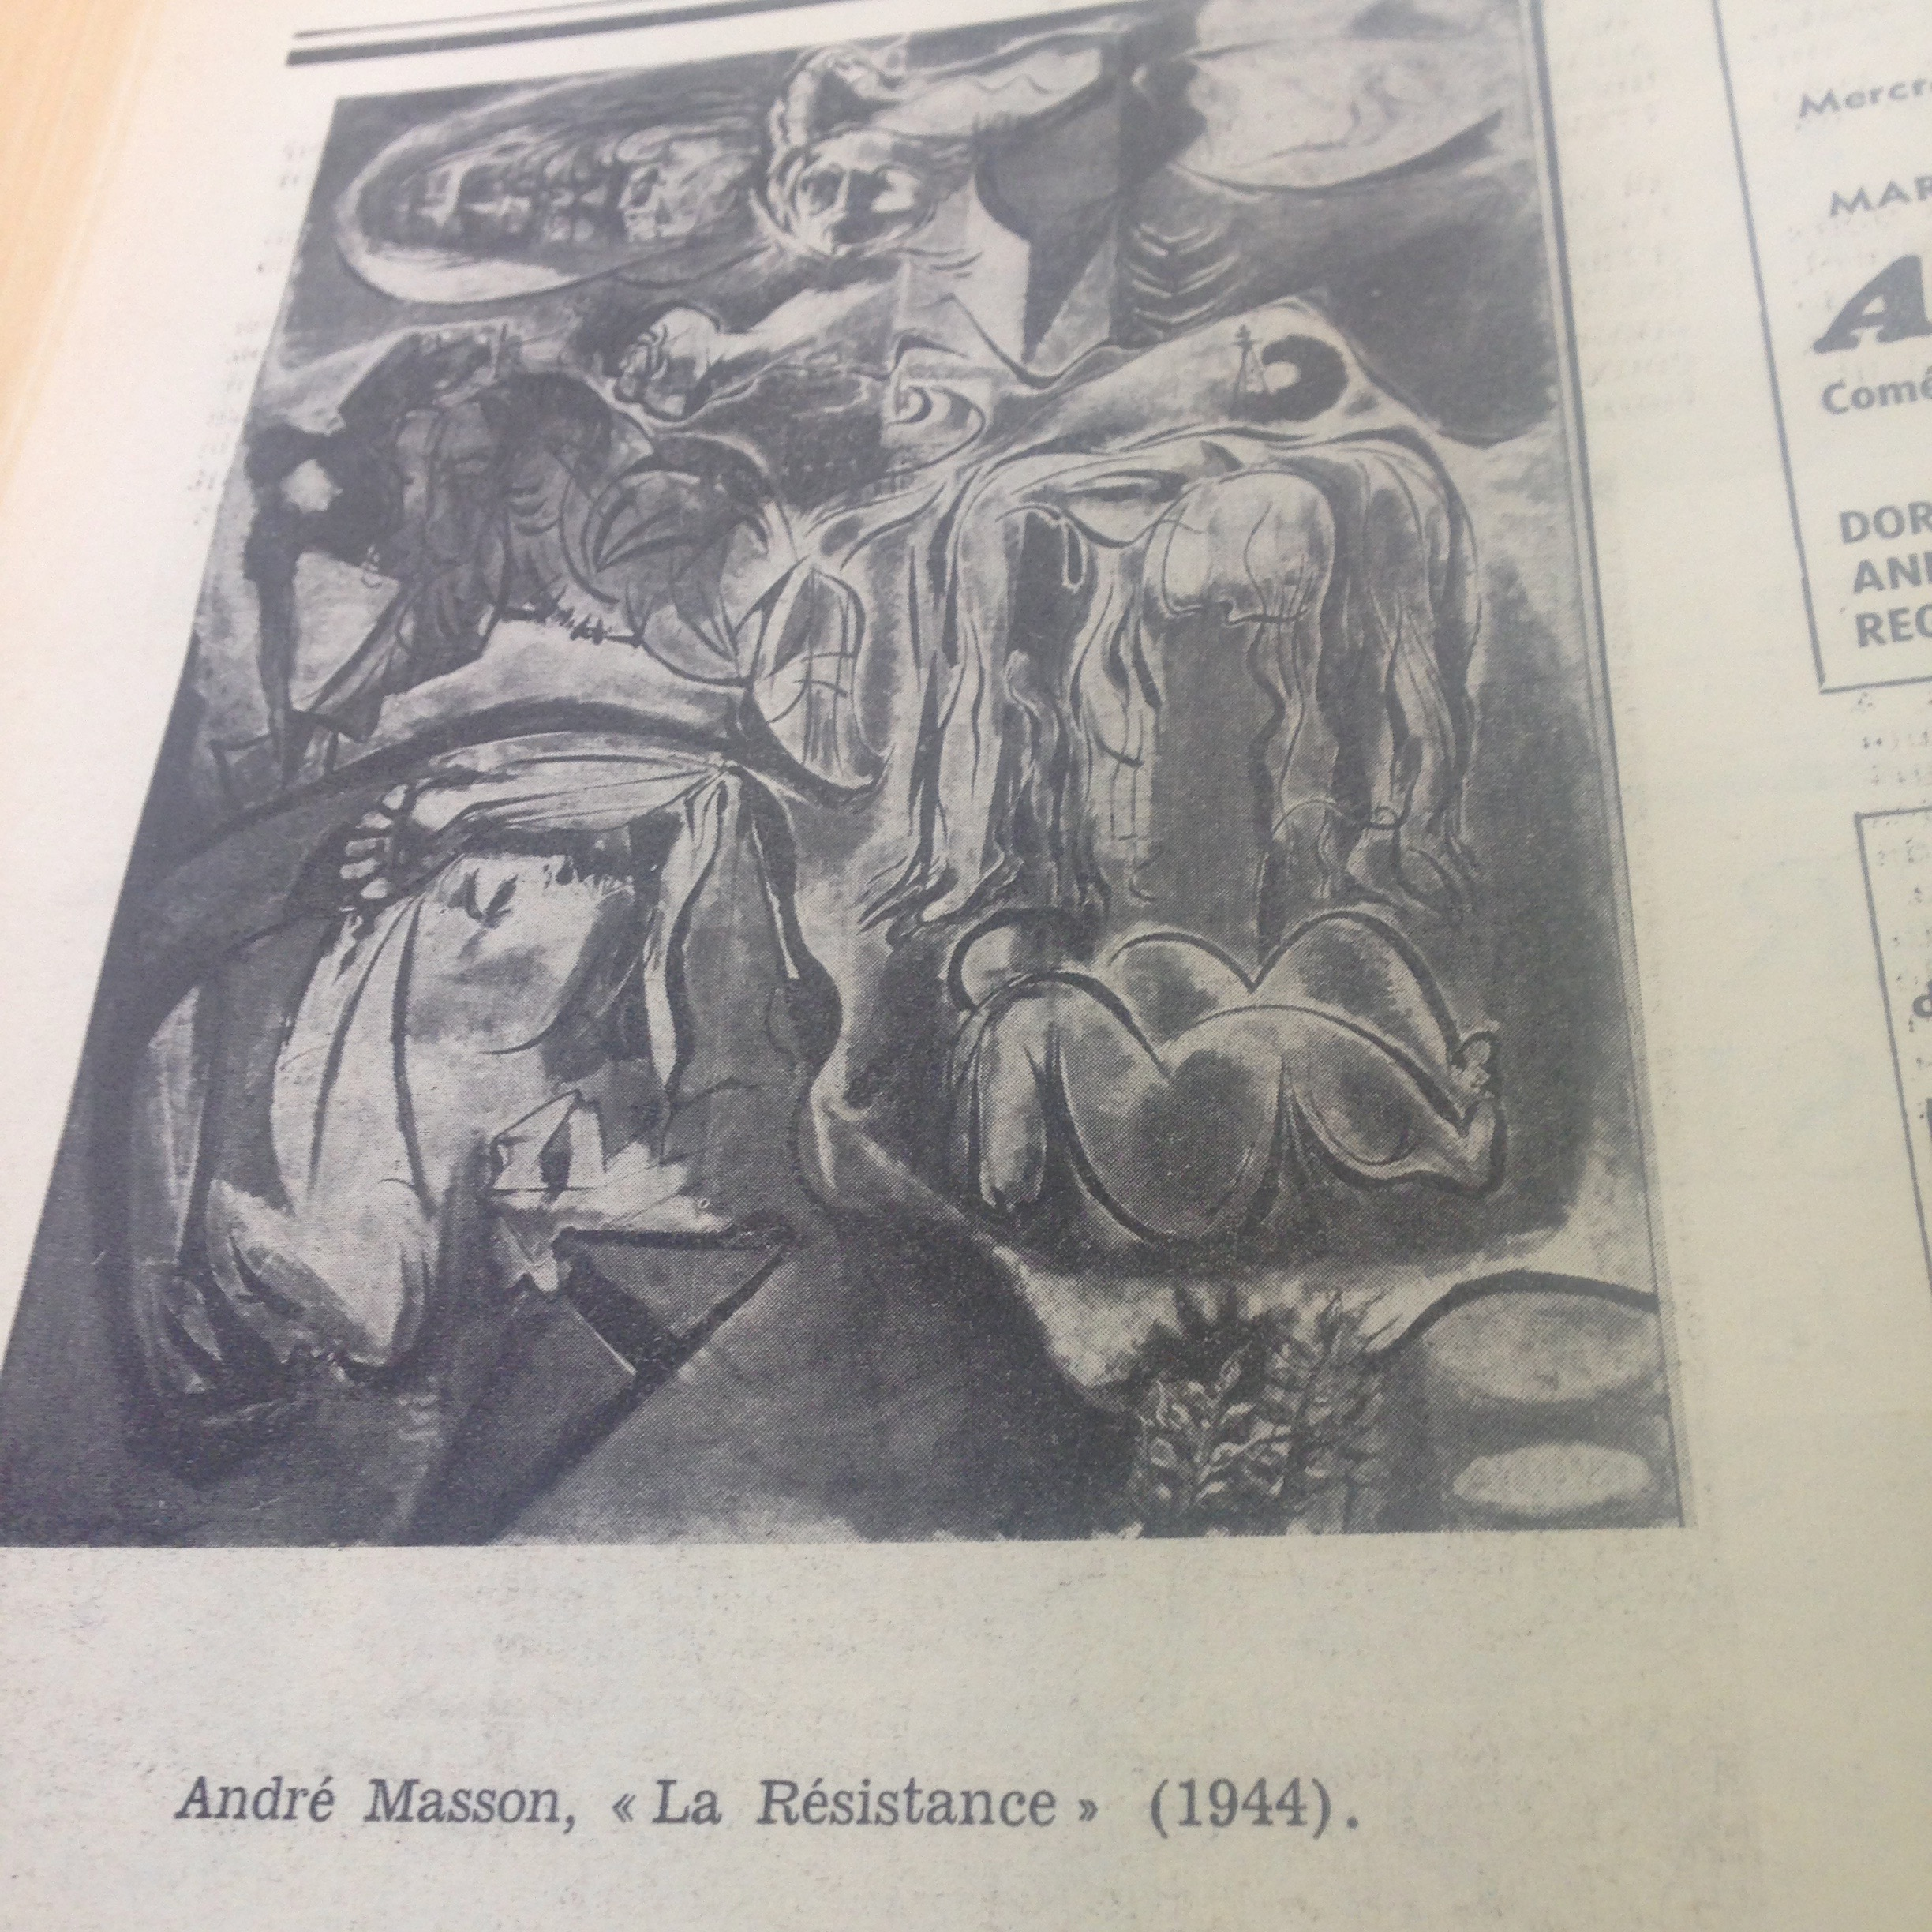
\includegraphics[width=0.33\textwidth]{resistancep2.jpg}
	\caption{\cite{specialelsa}}\label{fig:Resistance}
\end{figure}

\begin{figure}[H]
   \centering
   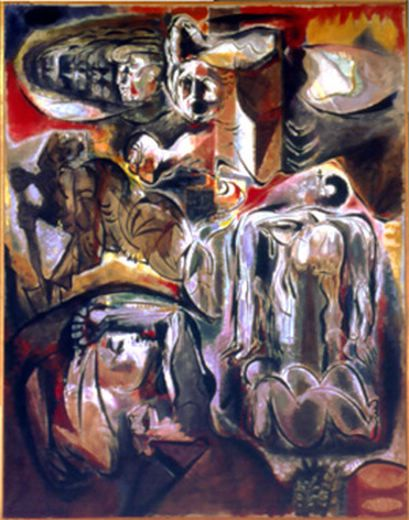
\includegraphics[width=0.33\textwidth]{resistancecouleur.jpg}
	\caption{\cite{specialelsa}}\label{fig:Resistancecouleur}
\end{figure}


C’est d’ailleurs à une troisième période historique auquel renvoie ce tableau de Masson, bien que le sujet ne serait pas immédiatement identifiable sans le titre et la date qui ne laisse pas le doute possible. La figuration n’est d’ailleurs pas plus immédiatement reconnaissable, et il faut s’attarder sur le tableau pour que se devinent derrière les formes apparemment géométriques et flasques le contour de fragments de corps de femme (bas de la toile) et de l’homme barbu qui lui est symétriquement opposé. En fait, on pourrait même se demander si le tableau ne se lit pas plutôt en format paysage. Quoi qu’il en soit, même avec la clarté du titre, le tableau demeure obscur, plus proche de l’énigme à déchiffrer. En outre, en reproduisant le tableau en noir et blanc, en sachant qu’il est arrivé en particulier dans ces années-là au journal de faire des reproductions en couleur, on peut supposer que l’enjeu n’est pas seulement financier mais stratégique : Si on retire les couleurs vives de ce tableau qui imprègnent directement l’attention, l’observateur revient comme souvent sur les formes. Un tel choix se justifie d’autant plus avec le recours au nombreux dessins et surtout esquisses pour les oeuvres d’André Masson en particulier. Sans compter qu’André Masson lui-même est une figure médiatrice particulièrement indiquée pour associer la Commune de Paris de 1871 et Elsa Triolet. D’une part, nous avons eu l’occasion d’analyser l’article \emph{André Masson et la Commune}\footcite{commune} par  Raoul-Jean Moulin avec le témoignage intime et des esquisses du peintre. D’autre part, André Masson avait été l’un des participants à la mémoire d’Elsa Triolet dans le fameux numéro après sa mort en Juin 70, intitulé \emph{Elsa}\footcite{specialelsa}. Son hommage était assez atypique, même vis-à-vis des autres peintres, puisqu’il avait choisi de ne pas écrire de texte pour lui dédier l’un de ses plus fameux  tableaux sur la femme, \emph{Mélusine}. Comprendre la démarche éditoriale et la fonction symbolique qu’y incarne le tableau Résistance de Masson, c’est donc d’abord avoir en mémoire cet autre numéro au moment de la mort d’Elsa, publié dans les plus vives émotions de la perte.


C’est pourquoi, paradoxalement au sujet du tableau, André Masson opère nécessairement d’abord le lien entre deux imaginaires proprement romantiques chez Aragon, la Commune de Paris et la figure d’Elsa. Il n’est pas anodin que, plus que pour aucun autre événement historique, les numéros des \emph{Lettres françaises} constituent une abondante réserve historique de documents sur ce moment de l’Histoire en particulier. Pas plus que prolonger après une première partie sur l’\emph{Après-dire} d’Aragon pour les \emph{ORC} de \emph{Blanche ou l’oubli} où Aragon y exprime l’égarement après la perte d’Elsa, la seconde partie du numéro porte sur l’Histoire de la Commune. Il apparait ainsi que la stratégie éditoriale du journal dirigé par Aragon n’est pas uniquement d’ordre politique et idéologique, comme on a pu le voir dans des exemples précédents, mais aussi d’ordre purement intime. 


	Pourtant, c’est avant tout l’aspect de la rigueur historique qui prédomine dans ce rassemblement d’études d’auteurs sur la Commune. Pas forcément à l’avantage de celle-ci, si l’on pense à l’ouvrage de Jacques Rougerie,\emph{Procès des communards}, plus proche de la désillusion. Si l’image de Louise Michel reste brave, le livre montre aussi qu’elle est plus une exception qu’un exemple, et l’on assiste aux revirements d’opinions de nombreux communards au moment du jugement. Si la Commune est vécue par \emph{Les Lettres françaises} avec une passion sans bornes, depuis 51, à travers la figure de Courbet, ce n’est pas tant par l’idéalisation de la figure romantique du communard révolutionnaire, mais par une démarche plutôt scientifique qui trahit l’obsession du journal pour cet événement historique en particulier : \enquote{Jamais peut-être encore n’a-t-on tant publié de livres pour un anniversaire} introduit la direction en guise de préface à l’entretien, ce à quoi Pierre Daix pose une problématique claire autour de ces quatre ouvrages : \enquote{Comment écrire l’histoire de la Commune en 1971 ?} Or, ce qui ressort le plus précisément de l’entretien animé par Pierre Daix, c’est le point commun de ces quatre auteurs et historiens à aborder les sources sur la Commune non du point de vue de ses grands représentants, mais plutôt du peuple. Et le dessein de ce projet, Jean Bruhat le souligne, et l’on comprend combien il s’imbrique dans la politique culturelle du journal : \enquote{il y aurait beaucoup à rechercher à propos du retentissement de la Commune sur les mentalités ouvrières.}
	Plus qu’aucune autre période historique, le journal a recueilli tellement de documents d’archives sur la Commune que Les Lettres Françaises peut se considérer sur l’ensemble des numéros depuis 51 comme une anthologie de l’Histoire de la Commune de Paris. On peut même y ajouter à cela un autre sujet apparemment distinct et dont pourtant son aspect romantique vient du souvenir de la Commune : Lorsqu’un numéro publie des photos du quartier de Belleville, le souvenir de la Commune n’est pas étranger à cette nostalgie pour ce quartier du XXème. Tout particulièrement dans les années 70 où les numéros déplorent l’architecture de Paris en train de se modifier, perdre une âme d’origine. L’immense article reproduit d’ailleurs un plan de la ville de Paris avant les travaux d’Haussmann. Or, c’est justement la question de l’héritage de la pensée communarde qui réunit les quatre historiens : Son héritage sur les ouvriers d’aujourd’hui d’une part, celle qu’en fit sa digne héritière la révolution de 1917 d’autre part. 


André Masson, le médiateur du numéro, est également mentionné dans la légende du livre de Georges Soria, \emph{La grande histoire de la Commune}, dont l’un des dessins illustre ce grand entretien. Sa position aux côtés du sommaire prête ainsi un autre sens à la période bien précise de la Résistance sous la Seconde Guerre Mondiale. Résistance devient par cette place de choix de présentation du numéro comme la résistance des \enquote{communeux}, qui défendent les barricades de la ville de Paris conte l’armée versaillaise pendant 73 jours. C’est peut-être aussi ce qui explique le choix de la direction des \emph{tLettres françaises} de choisir le tableau de Masson plutôt qu’une photographie de la Commune ou un peintre à l’esthétique plus mimétique : L’énigme qui ressort de cette toile n’évoque pas tant une période historique que la recherche du sens le plus absolu possible du terme \enquote{résistance}. On discerne d’ailleurs difficilement des visages, hormis celui de la jeune femme du bas de la toile, levant un poing musclé plutôt masculin. Elle est opposée symétriquement à l’homme barbu du haut de la toile, dans une attitude plus pensive. Dans ce méli-mélo de fragments de corps, la résistance est avant tout la propre révolte du peintre. Car c’est peut-être là une conception commune à Aragon et Masson, celle de concevoir dans le processus de la résistance la nécessité pour advenir de la révolte.

	 Ainsi, on aurait pu s’attendre à la lecture de l’entretien mené par Pierre Daix à une représentation du peuple, communard ou d’une autre nature révolutionnaire.  Mais, devant l’orientation de l’entretien, à laquelle Pierre Daix en tant qu’animateur n’est pas étranger, recherche à retrouver l’esprit du peuple parisien communard. Et plus, précisément, comment s’exprime l’état d’esprit du peuple communard. C’est au titre de cette recherche d’expression de la pensée observée par un regard contemporain que ce grand entretien entre les historiens et Pierre Daix rejoint la nature de la composition de la \emph{Résistance} d’André Masson. Sans compter que, chez Masson, l’expression est à la fois individuelle et inscrite dans l’histoire des hommes. On peut en vouloir pour preuve le sujet que prépare André Masson en vue d’une conférence en 1939 en Amérique :
\begin{quote}
En voici  à peu près le thème : “Quel est le mobile profond qui pousse un homme à se livrer à se livrer  à l’expression artistique ? , dans quelle mesure peut-il apporter aux autres hommes embrouillés comme lui dans l’enchevêtrement de la vie une représentation qui résiste un peu au chaos, au devenir.“ Je pose comme vous le voyez le problème et mon point de départ est d’ordre “ontologique“ ».\footcite[p259]{rebelle} \end{quote}
 
	En somme, \emph{Résistance}, chez Masson, comporte cette notion métaphysique chère à son collectionneur Kahnweiler. Et, même à ce niveau, l’acte de résistance s’entrecroise avec celui de révolte. C’est particulièrement observable dans une telle toile où, jusque dans sa forme infixable, sa lecture multiple, la résistance est également intérieure. Il est donc extrêmement révélateur que la direction, peut-être un choix d’Aragon lui-même dans ce numéro majeur où il exprime son propre deuil, traduise l’expression de sa tourmente intérieure par ce tableau de Masson. En somme, Résistance n’établit pas uniquement une médiation entre la figure de Paris et la Commune de Paris, la recherche commune de la trace de l’expression du peuple, mais la mise-en-page le choisit comme médiateur entre Aragon et Elsa Triolet. Ce qui, compte tenu de l’amitié forte qui l’unissait à cette dernière de son vivant, ce qu’ont démontré plus d’un numéro des Lettres françaises en les associant, est symbolique des réelles relations du couple vis-à-vis d'André Masson. 